\documentclass[12pt, a4paper, openany]{book}
\usepackage[inline]{enumitem}
\usepackage{../generalStyle}
\usepackage{graphicx}
\usepackage{float}
\usepackage{amsmath}
\usepackage{hyperref}

\hypersetup{
    pdftitle={Formulario di Fisica},
    pdfsubject={Formulario di Fisica dalla Cinematica all'Elettromagnetismo},
    pdfauthor={Gianluca Parpanesi},
    pdfkeywords={Formulario}
}



\begin{document}

\title{Formulario di Fisica}
\author{Gianluca Parpanesi}
\date{2022/2023}
\maketitle

\section*{Prefazione}

Questo formulario ha l'intenzione di fornire tutte le nozioni teoriche base ai 
fini di comprendere al meglio le formule qui riportate.
Ogni argomento e ogni formula trattata sono precedute da una breve spiegazione
teorica.
Per chi desiderasse avere un riassunto conciso con le sole formule, può 
trovarlo in fondo al formulario.
    \subsection*{Argomenti trattati}
    Gli argomenti trattati in questo formulario si basano sul corso di Fisica 
    frequentato a settembre 2022 della facoltà di Informatica. Gli argomenti
    trattati sono i seguenti:
    \begin{itemize}
        \item Meccanica Classica
        \begin{itemize}
            \item Cinematica 
            \item Dinamica
            \item Energia e Lavoro
            \item Moto Armonico e Oscillazioni
        \end{itemize}
        \item Gravitazione 
        \item Fluidodinamica
        \item Termodinamica
        \item Magnetismo
        \item Elettrostatica
        \item Elettromagnetismo
        \item Circuiti
    \end{itemize}

    \subsection*{Materiale di riferimento}
    Il libro adottato come riferimento per questo formulario è 
    l'Halliday-Resnick Fondamenti di Fisica (Jearl Walker), Edizione 7, Casa 
    Editrice Ambrosiana (Volume 1 e 2)

\newpage

\tableofcontents
\newpage

\section*{Nozioni Generiche}

\begin{itemize}
    \item La velolcità di un corpo è identificata come lo spostamento sul tempo
    :
        \begin{equation*}
            v = \frac{dx}{dv}
        \end{equation*}
    \item L'accelerazione di un corpo è identificata come la velocità sul tempo
    :
        \begin{equation*}
            a = \frac{dv}{dt}
        \end{equation*}
    \item La massa non influisce sul tempo di caduta dovuto da un campo 
        gravitazionale. Due oggetti con masse completamente diverse subiscono 
        la stessa identica accelerazione.
    \item Una forza è conservativa se il lavoro netto che una particella compie
    in un percoso chiuso è 0. In modo equivalente, una forza è conservativa 
    se il Lavoro netto che compie una particella in movimento non dipende dal 
    percorso che essa compie. La forza gravitazionale e la forza elastica sono
    forze conservative, l'attrito dinamico non è una forza conservativa.
    
    \paragraph{Prodotto tra vettori} Il prodotto tra due vettori può essere 
    eseguito in due modi differenti: il primo tipo di prodotto dà origine ad 
    uno scalare (prodotto scalare) mente l'altro darà origine ad un vettore 
    (prodotto vettoriale).
    \begin{itemize}
        \item \textbf{Prodotto scalare}: il prodotto scalare dei vettori $a$ e
        $b$ si scrive $a \cdot b$ ed è definito dall'espressione
        \begin{equation*}
            a \cdot b = ab \cos \Theta
        \end{equation*}
        dove $a$ è il modulo del vettore $\boldsymbol{a}$, $b$ il modulo del 
        vettore $\boldsymbol{b}$ e $\Theta$ è l'angolo formato dalle semirette 
        equiverse su cui giacciono i due vettori.
        \item \textbf{Prodotto vettoriale}: il prodotto vettoriale 
        dei vettori $a$ e $b$ si scrive $a \times b$ ed è definito 
        dall'espressione
        \begin{equation*}
            a \times b = ab \sin \Theta
        \end{equation*}
        dove $a$ è il modulo del vettore $\boldsymbol{a}$, $b$ il modulo del 
        vettore $\boldsymbol{b}$ e $\Theta$ è il minore dei due angoli formati 
        dalle semirette equiverse su cui giacciono i due vettori. 
        La direzione del vettore risultante è \textbf{perpendicolare} al piano 
        individuato da $a$ e $b$.
    \end{itemize}
    
\end{itemize}

\chapter{Cinematica}

    \section{Moto rettilineo uniforme}

        \paragraph{Velocità} 
            La velocità viene rappresentata da uno scalare:
            \begin{equation}
                v_x = k
            \end{equation}

        \paragraph{Velocità media} 
            La velocità media viene rappresentata come un intervallo di uno 
            spostamento su un intervallo di tempo:
            \begin{equation}
                v_m = \frac{\Delta x}{\Delta t} = \frac{x_f - x_i}{t_f - t_i}
            \end{equation}

        \paragraph{Velocità istantanea} detta anche semplicemente velocità di 
        una particella, è definita come:
            \begin{equation}
                v = \lim_{x \to 0}  \frac{\Delta x}{\Delta t} = \frac{dx}{dt}
            \end{equation}

        \paragraph{Spostamento}
            \begin{equation}
                x(t) = x_i + v_xt
            \end{equation}

    \section{Moto uniformemente accelerato}

        \paragraph{Accelerazione media} è il rapporto fra la variazione della
        velocità $\Delta v$ che avviene in un intervallo di tempo $\Delta t$, 
        definita come:
        \begin{equation}
            a_m = \frac{\Delta v}{\Delta t} = \frac{v_f - v_i}{t_f - t_i}
        \end{equation}

        \paragraph{Accelerazione istantanea} o semplicemente accelerazione, è 
        la rapidità di variazione della velocità. Matematicamente si tratta 
        della derivata seconda della posizione $x(t)$ rispetto al tempo:
        \begin{equation}
            a = \frac{dv}{dt} = \frac{d^2x}{dt^2}
        \end{equation}

        \paragraph{Spostamento}
            \begin{equation}
                x(t) = x_i + v_it + \frac{1}{2}at^2
            \end{equation}

        \paragraph{Velocità finale}
            \begin{equation}
                v_f(t) = v_{i} + at
            \end{equation}
    
        \paragraph{Caso particolare}
            Per determinare il tempo possiamo effettuare la fomrula inversa 
            dello spostamento. È possivile notare come il tempo non dipende 
            dalla massa degli oggetti, ma dall'altezza e dalla forza di gravità
            . In assenza d'aria di conseguenza due oggetti con masse 
            completamente diverse arrivano a terra allo stesso tempo!

            \begin{equation}
                t_c=\sqrt{\frac{2h}{g}}
            \end{equation}

    \section{Moto di un proiettile} 

        Il moto di un proiettile è scomponibi le lungo gli assi cartesiani in 
        due moti ben distinti, agenti su un unico corpo:
        \begin{itemize}
            \item \textbf{Asse X}: moto rettilineo uniforme.
            \item \textbf{Asse Y}: moto rettilineo uniformemente accelerato.
        \end{itemize}
        Soffermandoci su questo ragionamento possiamo notare come la forza di 
        gravità (accelerazione) agisca in modo costante lungo l'asse y 
        effettuando un'accelerazione negativa (decelerazione) lungo questa 
        componente del moto. Il moto dell'asse x invece non viene intaccato da 
        nessun'altra forza (trascurando ovviamente l'attrito dell'aria).
        
        \paragraph{Equazioni del moto}
        (Per assi cartesiani)
        \begin{align}
            x &: x(t) = x_0 + v_{0x}t \\
            y &: \begin{cases}
                    y(t) &= y_0 + v_{0y}t + \frac{1}{2}at^2 \\
                    v_{fy} &= v_{0y} + at
                \end{cases}
        \end{align}

    \section{Moto circolare uniforme}
        Nel moto circolare uniforme agiscono 3 forze:
        \begin{itemize}
            \item Velocità tangenziale
            \item Accelerazione centripeta
            \item Accelerazione centrifuga
        \end{itemize}
        Le prime due sono forze fisiche reali, mentre la terza è chiamata forza
        apparente. Difatti la forza che ci fa sentire spinti verso l'esterno è
        data dalla nostra inerzia nel tendere a proseguire il nostro moto 
        diritti, mentre l'accelerazione centripeta (sempre rivolta verso il
        centro della curva) ci tiene in traiettoria circolare. Questo accade
        perché ci troviamo in un sistema non inerziale: difatto se lanciassimo 
        una pallina mentre ci troviamo all'interno di un moto circolare essa ci
        sembrerà allontanarsi da noi con una sua traiettoria, spinta da una 
        forza (apparente) verso l'esterno. Vista da un osservatore posto al di
        fuori del moto (in un sistema inerziale) semplicemente la pallina 
        proseguirà diritta nella sua traiettoria.\\\\
        Analizziamo ora le formule del moto circolare uniforme:

        \paragraph{Velocità tangenziale} La velocità tangenziale è lo spazio 
        percorso dal punto materiale in un intervallo di tempo:
        \begin{equation}
            v = \frac{2\pi r}{T}
        \end{equation}

        \paragraph{Accelerazione centripeta} L'accelerazione centripeta è 
        quella forza che mantiene un corpo in un moto circolare uniforme. Essa
        è sempre diretta verso il centro della circonferenza!.
        \begin{equation}
            a_c = \frac{v^2}{r}=
        \end{equation}
        Come vedremo più avanti in questo formulario l'accelerazione è impressa
        da una forza agente sul corpo, descrivibile (tramite la Seconda Legge
        di Newton) come:
        \begin{equation}
            F_{accelerazione} = ma = m\frac{v^2}{r}
        \end{equation}

        \paragraph{Periodo} Il tempo richiesto perché una particella completi
        una circonferenza è:
        \begin{equation}
            T = \frac{2\pi r}{v}
        \end{equation}

    
        \subsection{Moto Armonico}  \label{moto_armonico}
        Il moto circolare uniforme può essere scomposto in due moti sinusoidali 
        $\sin$ e $\cos$.
        Il moto circolare uniforme e quello uniformemente accelerato possono 
        essere perfettamente paragonati al moto rettilineo uniforme e quello 
        uniformemente accelerato. In questo caso $\Theta$ è la nostra $x$ 
        mentre la velocità $v$ diventa $\omega$.\\\\
        Nel caso uniformemente accelerato l'accelerazione $a$ diventa $\alpha$.

        \paragraph{Legge oraria (equazione del moto)} Essa descrive il moto del
        moto circolare uniforme, espresso come angolo in funzione del tempo:
        \begin{equation}
            \Theta = \Theta_0 + \omega t = 
            \begin{cases}
                x(t)=R\cos{\Theta(t)} \\
                y(t)=R\sin{\Theta(t)}
            \end{cases} 
            = 
            \begin{cases}
                x(t)=R\cos{(\Theta_o+\omega t)} \\
                y(t)=R\sin{(\Theta_o+\omega t)}
            \end{cases}
        \end{equation}

        \paragraph{Velocità angolare} La velocità angolare è l'angolo percorso
        dal punto materiale in un intervallo di tempo:
        \begin{equation}
            \omega = \frac{2\pi}{T}
        \end{equation}
        Espressa in radianti al secondo.

        \paragraph{Velocità tangenziale} La velocità tangenziale è lo spazio 
        percorso dal punto materiale in un intervallo di tempo:
        \begin{equation}
            v = \frac{2\pi r}{T} = 
            \begin{cases}
                v_x=-R\omega\sin{(\Theta_o+\omega t)} \\
                v_y=R\omega\cos{(\Theta_o+\omega t)}
            \end{cases}
        \end{equation}

        \begin{quote}
            Da notare come (per definizione) le equazioni della velocità non 
            sono altro che la derivata ' dell'equazione del moto 
            (Legge oraria)! 
        \end{quote}

        \paragraph{Accelerazione centripeta} L'accelerazione centripeta è 
        quella forza che mantiene un corpo in un moto circolare uniforme. Essa
        è sempre diretta verso il centro della circonferenza!.
        \begin{equation}
            a_c = \frac{v^2}{r}=
            \begin{cases}
                a_x=-R\omega^2\cos{(\Theta_o+\omega t)} \\
                a_Y=-R\omega^2\sin{(\Theta_o+\omega t)}\end{cases}
        \end{equation}

        \begin{quote}
            Da notare come (per definizione) le equazioni dell'accelerazione 
            non sono altro che la derivata " dell'equazione del moto 
            (Legge oraria)! 
        \end{quote}
        
    \section{Moto circolare uniformemente accelerato} Nel moto circolare 
    uniformemente accelerato entra in gioco l'accelerazione totale come somma
    vettoriale dell'accelerazione centripeta e dell'accelerazione tangeziale.
    Di conseguenza l'equazione del moto sarà il sistema:

        \paragraph{Legge oraria (equazione del moto)}
        \begin{equation}
            \begin{cases} 
                \Theta = \Theta_0 + \omega_0t + \frac{1}{2}\alpha t^2 \\ 
                \omega = \omega_0+\alpha t
            \end{cases}
        \end{equation}

        \subsection{Tabelle di riepilogo} Di seguito sono riportate due tabelle 
        contententi un riepilogo delle formule (comprese le formule inverse) 
        sia del Moto circolare uniforme \ref{fig:MCU} che del Moto circolare 
        uniformemente accelerato \ref{fig:MCUA}.

        \begin{figure}[H]
            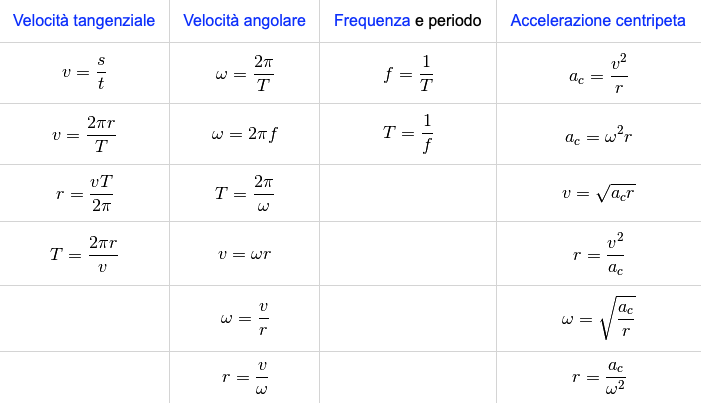
\includegraphics[width=0.9\linewidth]
            {formulario/img/Formulario_MCU.png}
            \caption{Formule del Moto circolare uniforme}
            \label{fig:MCU}
        \end{figure}

        \begin{figure}[H]
            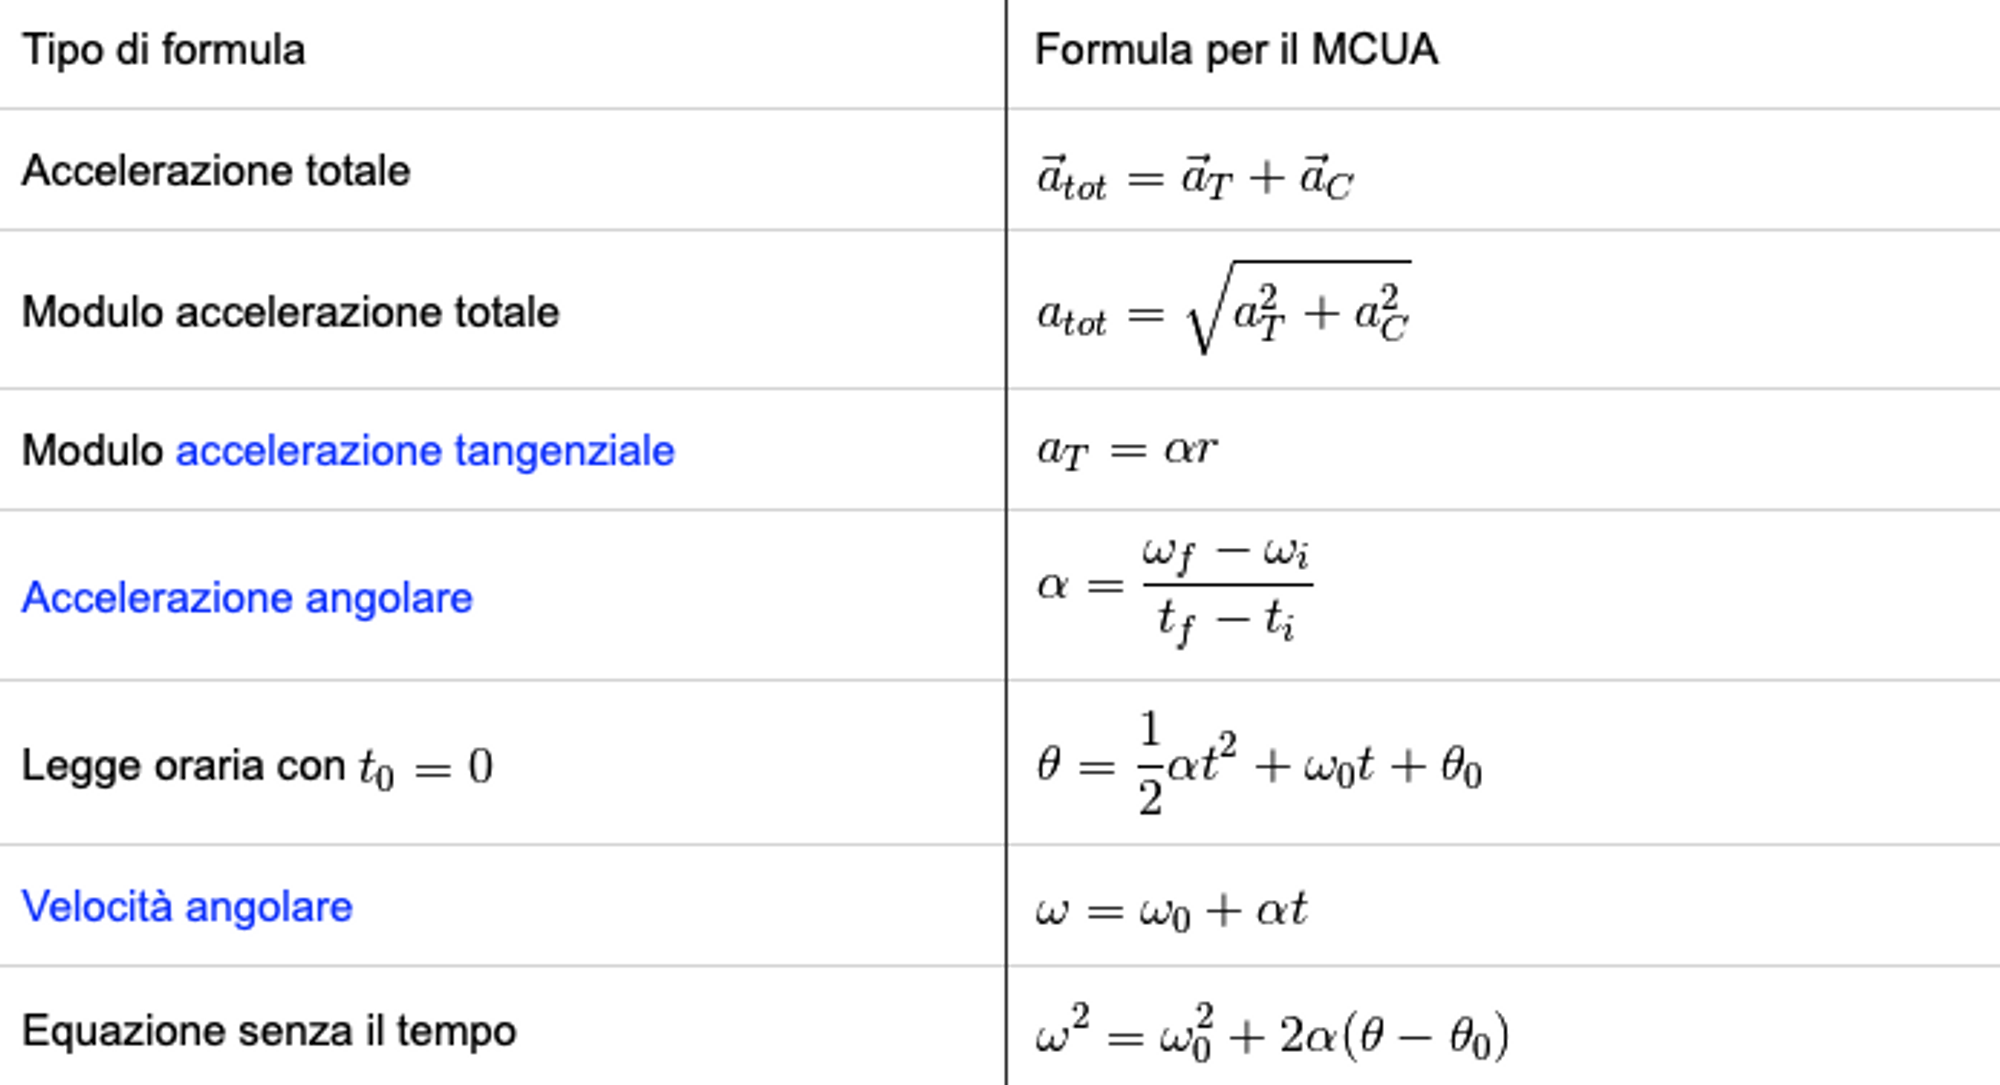
\includegraphics[width=0.9\linewidth]
            {formulario/img/Formulario_MCUA.png}
            \caption{Formule del Moto circolare uniformemente accelerato}
            \label{fig:MCUA}
        \end{figure}

        

\chapter{Dinamica}

    \section{Principi della Dinamica - Leggi di Newton}

        \paragraph{Prima Legge di Newton} Se la somma delle forze che agiscono 
        su un corpo è nulla, allora il corpo in quiete rimarrà in quiete, mentre
        se è in moto, continuerà a muoversi di moto rettilineo uniforme.

        \paragraph{Seconda Legge di Newton} La forza agente su un corpo è 
        direttamente proporzionale all'accelerazione e ne condivide la direzione
        e il verso, ed è direttamente proporzionale alla massa. Di contro 
        l'accelerazione cui è soggetto il corpo è direttamente proporzionale 
        alla forza e inversamente proporzionale rispetto alla massa.

        \begin{equation}
            \vec{F} = m \vec{a} \; [N]
        \end{equation}

        \paragraph{Terza Legge di Newton} Se un corpo A esercita una forza su 
        un corpo B, allora il corpo B esercita su A una forza uguale e 
        contraria.

        \begin{equation}
            F_{ab} = - F_{ba}
        \end{equation}

        \begin{quote}
            Attenzione! Le forze hanno modulo uguale ma con segno vettoriale 
            opposto!
        \end{quote}

    \section{Forza Elastica} La forza elastica di un corpo (o di una molla) è 
    descritta dalla Legge di Hook nel seguente modo:
        \begin{equation}
            F = -kx
        \end{equation}
    Dove $-k$ è chiamata \textbf{costante elastica} ed è una misura della 
    rigidità della molla. Maggiore è $k$, più rigida è la molla: cioè maggiore è
    $k$, maggiore sarà la forza per uno stesso valore di spostamento.

    \section{Carrucola} Le forze agenti su due corpi collegati in un sistemma a
    carrucola (se aventi masse diverse) sono sempre una l'opposta dell'altra.
        \begin{equation}
            \begin{cases}
                F_{y1} = T - m_1g \\
                F_{y2} = m_2g - T
            \end{cases}
        \end{equation}
    In questo caso si considera $m_2 > m_1$ e con un sistema di riferimento 
    verticale. Si considera infatti un sistema a carrucola con forze agenti solo
    sull'asse $y$ e con forze nulle sull'asse $x$.

    \section{Attrito Statico e Dinamico} La forza di attrito è una forza che 
    agisce in direzione opposta allo spostamento (opponendosi al movimento). La 
    forza di attrito può agire in due modi differenti:
        \begin{itemize}
            \item \textbf{Attrito statico}: agente quando il corpo è fermo, 
            impedendo lo spostamento iniziale.
            \item \textbf{Attrito dinamico}: agente da quando il corpo ha appena 
            compiuto lo spostamento iniziale ed è in movimento.
        \end{itemize}
    Le formule sono per l'attrito statico:
        \begin{equation}
            f_{s, max} = \mu_sF_N
        \end{equation}
        Mentre per quello dinamico:
        \begin{equation}
            f_{k} = \mu_kF_N
        \end{equation}
    
    \section{Resistenza di un corpo} Quando un corpo solido si muove 
    all'interno di un fludio, ad esso si oppone una forza contraria chiamata
    resistenza $D$ la quale farà raggiungere al corpo una velocità massima:
        \begin{equation}
            D = \frac{1}{2}CA\rho v^2
        \end{equation}
        Con:
        \begin{itemize}
            \item C : Coefficiente di resistenza aerodinamica.
            \item A : Area efficace della sezione trasversale del corpo.
            \item $\rho$ : densità dell'aria
            \item v : velocità.
        \end{itemize}

    \section{Lavoro} Si applichi una forza F ad un oggetto per spostarlo. La 
    Forza sarà tanto efficace ad ottenere uno spostamento \textbf{tanto più
    è applicata nella stessa direzione dello spostamento.}

        \begin{equation}
            W = Fd = Fd \cos \Theta \; [J]
        \end{equation}

        \paragraph{Lavoro compiuto dalla Forza Gravitazionale} Il Lavoro svolto 
        dalla Forza Gravitazionale ovviamente è descritto come $F d$, per un 
        corpo che sale la $F_g$ è diretta in senso opposto allo spostamento 
        formando un angolo $\Theta$ di $180^{\circ}$.
        
        \begin{equation}
            F = mgd\cos \Theta = mgd \cos 180 = - mgd
        \end{equation}
        Mentre nel momento in cui un corpo cade, la $F_g$ avrà stessa direzione
        dello spostamento (verso il basso), conferendo un segno positivo al
        Lavoro.
        
        \paragraph{Lavoro compiuto dalla Forza Elastica} La Forza Elastica non è
        una forza costante e di conseguenza non possiamo utilizzare la classica
        equazione del Lavoro (per una forza costante). Possiamo però suddividere
        lo spostamento della molla in parti infinitesime in modo da avere forze
        infinitesime per ogni spostamento infinitesimo, facendo risultare cosi 
        la forza infinitesima costante su uno spostamento infinitesimo. 
        Integrando questa operazione otterremo così la formula del lavoro per
        la Forza Elastica (e in generale per una forza non costante!).
        \begin{equation*}
            L_m = \int_{x_f}^{x_i} -F \,dx 
        \end{equation*}
        \begin{equation*}
            L = \int_{x_f}^{x_i} -kx \,dx =  L = -k \int_{x_f}^{x_i} x \,dx   
        \end{equation*}
        \begin{equation*}
            = (-\frac{1}{2}k)\bigg[x^2 \bigg]_{x_f}^{x_i}
            = (-\frac{1}{2}k) (x^2_f - x^2_i)
        \end{equation*}
        \begin{equation}
            L_m = \frac{1}{2}kx^2_i - \frac{1}{2}kx^2_f
        \end{equation}
        Il Lavoro $L_m$ è positivo quando il blocco si avvicina alla posizione 
        di riposo $x=0$ ed è negativo quando se ne allontana. Il Lavoro è nullo
        se la distanza finale da $x=0$ non è mutata.

    \section{Energia Cinetica} Rappresenta la quantità di energia associata al 
        moto di una particella (corpo puntiforme) che si muove alla velocità $v$.

        \begin{equation}
            K = \frac{1}{2}mv^2 \; [J]
        \end{equation}

        \begin{quote}
            Il lavoro fatto su una particella è uguale a $\Delta K$. L'energia 
            cinetica (e la velocità) aumentano se il lavoro svolto è positivo, 
            mentre diminuiscono se il lavoro svolto è negativo.
        \end{quote}

        \paragraph{Teorema dell'Energia Cinetica} Chiamiamo $\Delta K$ la 
        variazione di Energia Cinetica del corpo e $L$ il Lavoro totale compiuto
        su di esso. Allora possiamo scrivere:
        \begin{equation}
            \Delta K = K_f - K_i = W
        \end{equation}

        \paragraph{Energia Cinetica del Moto Armonico Semplice} Si consideri un
        sistema molla-blocco, nel caso senza attriti, possiamo visualizzare il 
        suo andamento come un'oscillazione armonica e descrivere la sua Energia
        Cinetica come:
        \begin{equation}
            K = \frac{1}{2}mv^2 = \frac{1}{2}m\omega^2A^2\sin^2
            (\Theta + \omega t)
        \end{equation}

    
    \section{Potenza} Se una forza esterna è applicata ad un oggetto e se il 
    Lavoro è fatto in un intervallo di tempo, definiamo \textbf{potenza}:
        
        \begin{equation}
            P = \frac{W}{\Delta t} \; [W \textsf{  Watt}]
        \end{equation}

        \paragraph{Un altro sguardo alla Potenza} La Potenza Istantanea può 
        essere espressa derivando la formula della Potenza (ovviamente!). Di 
        conseguenza possiamo scrivere la potenza come:

        \begin{equation*}
            P = \frac{dL}{dt} = \frac{F \cos \Theta dx}{dv} 
            = F \cos \Theta (\frac{dx}{dt})
        \end{equation*}
        Ma sappiamo benissimo che $\frac{dx}{dv}$ non è altro che la definzione 
        di velocità. Possiamo quindi riscriverla in modo più semplice:
        \begin{equation*}
            P = Fv\cos\Theta
        \end{equation*}
        Ovvero il \textbf{prodotto scalare} tra $F$ e $v$ (dove $v$ è la 
        velocità della particella). Possiamo quindi scrivere che la Potenza 
        Istantanea di una paricella a velocità $v$ non è altro che:
        \begin{equation}
            P = F \cdot v
        \end{equation}

    \section{Energia Potenziale} Se la configurazione di un sistema cambia, 
    allora cambierà anche la sua Energia potenziale. Quando un oggetto si trova
    ad una certa distanza dal suolo, il sistema terra-oggetto ha un'energia 
    potenziale che si trasforma in lavoro. \\
    L'Energia Potenziale è associata con la configurazione del sistema nel quale
    le forze conservative agiscono. Quando una forza conservativa compie lavoro
    $W$ su una particella (corpo) del sistema, il cambiamento $\Delta U$ 
    dell'energia potenziale del sistema è definito come:
        
        \begin{equation}
            \Delta U = - W
        \end{equation}

        \paragraph{Energia Potenziale Gravitazionale} L'energia potenziale in un
        sistema composto dalla terra e dalla particella (corpo) è chiamata 
        Energia Potenziale Gravitazionale. Se la particella si muove da 
        un'altezza iniziale $y_i$ ad una finale $y_f$, il cambiamento 
        dell'Energia Potenziale Gravitazionale è definito come:
        \begin{equation}
            \Delta U = mg(y_f - y_i) = mg \Delta y
        \end{equation}
        Se considerassimo come punto di arrivo un altezza $= 0$, allora 
        l'Energia Potenziale gravitazionale piò essere riscritta come:
        \begin{equation}
            \Delta U(h) = mgh
        \end{equation}
        Dove $h$ è l'altezza dalla quale il corpo cade.

        \paragraph{Energia Potenziale Elastica} L'energia Potenziale Elastica è 
        l'energia associata allo stato di compressione o estensione di un 
        oggetto elastico (molla). Per una molla con una forza definita come 
        $ F = -kx $, l'Energia Potenziale Elastica sarà definita come:
        \begin{equation}
            U(x)     = \frac{1}{2}kx^2
        \end{equation}

        \paragraph{Energia Potenziale del Moto Armonico Semplice} L'energia 
        Potenziale Elastica di un oscillatore armonico, immagazzinata dalla 
        molla a seguito di un allungamento $x$ è:
        \begin{equation}
            U = \frac{1}{2}kx^2 = \frac{1}{2}kA^2\cos^2(\Theta + \omega t)
        \end{equation}

    \section{Energia Meccanica} La somma dell'Energia Cinetica e dell'Energia
    Potenziale è detta Energia Meccanica, definita come:

        \begin{equation}
            E_m = K + U
        \end{equation}

        \paragraph{Principio di conservazione dell'Energia Meccanica} Quando in 
        un sistema isolato agiscono solo forze conservative, l'Energia Cinetica 
        e l'Energia Potenziale prese singolarmente possono variare, ma la loro
        somma, l'Energia Meccanica $E_m$ del sistema non cambia. Questo 
        risultato è chiamato principio di conservazione dell'Energia Meccanica
        espirmibile nel seguente modo:
        \begin{equation}
            \Delta E_m = \Delta K + \Delta U = 0
        \end{equation}
        Il principio di conservazione dell'Energia Meccanica ci permette di 
        risolvere problemi che sarebbe arduo risolvere usando solo le Leggi di 
        Newton.
        Quando l'Energia Meccanica di un sistema si conserva, possiamo mettere
        in relazione il totale dell'Energia Cinetica e dell'Energia Potenziale
        in un istante con quello di un altro istante, \textit{senza dover
        considerare gli stati intermedi e senza necessità di conoscere il lavoro
        compiuto dalle forze coinvolte!}

        \paragraph{Principio esteso} La variazione dell'Energia Meccanica è 
        uguale al lavoro svolto dalle Forze non conservative:
        \begin{equation}
            \Delta E_m = W_{nc}
        \end{equation}
        

    \section{Moto Armonico e Pendolo} L'oscillatore armonico può essere 
    rappresentato da un sistema molla-blocco il quale oscillando descrive un 
    moto circolare uniforme. Le equazioni del moto sono le stesse del Moto 
    Circolare Uniforme \ref{par_mcu},
        \begin{equation}
            x(t) = A \cos(\Theta_0 + \omega t)
        \end{equation}
        ma con:
        \begin{equation*}
            \omega = \sqrt[]{\frac{k}{m}}
        \end{equation*}
        ricordando l'equazione dei un sistema molla-blocco:
        \begin{equation*}
            F = -kx
        \end{equation*}
        
        \paragraph{Il pendolo} Il pendolo può essere descritto tramite il
        Moto Circolare Uniformemente Accelerato, considerando la lunghezza del 
        filo inestensibile come il raggio della circonferenza. In questo caso 
        abbiamo:
        \begin{equation*}
            \omega = \sqrt[]{\frac{g}{L}}
        \end{equation*}
    
    
    
    \section{Momento Lineare}

        \begin{equation}
            p = mv
        \end{equation}

        \paragraph{Connessione con la II Legge di Newton} Deriviamo il 
        Momento Lineare rispetto al tempo. La derivata della quantità di moto di
        un punto materiale di massa $m$ è uguale alla risultante della forza 
        applicata.

        \begin{equation*}
            \frac{dp}{dt} = \frac{d(mv)}{dt} = ma
        \end{equation*}

        \begin{equation*}
            \frac{dm}{dt} v + m \frac{dv}{dt} = ma
        \end{equation*}

        \begin{quote}
            Ma la massa rimane costante nel tempo, quindi la derivata sarà 0.
        \end{quote}

        \begin{equation*}
            m\frac{dv}{dt} = ma = \sum F
        \end{equation*}

        \begin{equation*}
            \sum F = 0 \implies p = \textsf{cost}\
        \end{equation*}

        \paragraph{Legge di conservazione del momento lineare} Quando due o più
        particelle di un sistema isolato interagiscono, il momento lineare 
        totale del sistema resta \textbf{costante}.


    \section{Impulso}

        \begin{equation}
            I = F \Delta p
        \end{equation}

        \paragraph{Significato} L'impulso della forza che agisce su una 
        particella è aguale al $\Delta$ del momento lineare della particella 
        determinato dalla forza. L'impulso non è una caratteristica della 
        particella, bensì una misura della modifica del momento lineare da parte
         di una forza esterna.

        \paragraph{Connessione con il Momento Lineare} Sia una forza $F = F(t)$
        agente su una particella. Applicando la II Legge di Newton:

        \begin{equation*}
            F = \frac{dp}{dt} \implies dp = F dt
        \end{equation*}
        \begin{equation*}
            \Delta p = p_f - p_i = \int_{t_f}^{t_i} F \,dt = I 
        \end{equation*}
    
    \section{Urti} Gli urti accadono frequentemente nella vita quotidiana e 
    possono essere caratterizzati in due differenti tipi:
    \begin{itemize}
        \item \textbf{Urti elastici}: Se nell'urto tra due corpi l'Energia 
        Cinetica totale del sistema non cambia ma si conserva completamente.
        \item \textbf{Urti anaelastici}: L'Energia Cinetica non si conserva ma 
        parte viene dispersa in calore o suono (ad esempio).
    \end{itemize} 

        \paragraph{Urti Anaelastici} La collisione anaelastica comporta sempre
        una perdita di Energia Cinetica del sistema. La massima perdita si ha 
        quando i corpi si incollano insieme, in questo caso l'urto prenderà il 
        nome di \textbf{urto completamente anaelastico}.
        Un urto anaelastico può essere descritto tramite la seguente formula:
        \begin{equation}
            p_{1,i} + p_{2,i} = p_{1,f} + p_{2,f}
        \end{equation}
        ovvero:
        \begin{equation*}
            m_1v_{1,i} + m_2v_{2,i} = m_1v_{1,f} + m_2v_{2,f}
        \end{equation*}
        Nel caso di un \textbf{urto completamente anaelastico} uno dei due 
        corpi sarà inizalmente fermo (prendendo il nome di bersaglio). Dopo la 
        collisione proseguiranno attaccati con una velocità $V$. Definiamo 
        quindi l'equazione di un urto di questa tipologia:
        \begin{equation}
            m_1v_{1,i} = (m_1+m_2)V
        \end{equation} 
        \begin{quote}
            Abbiamo analizzato gli urti in una singola dimensione. In caso di 
            urti in due dimensioni le considerazioni appena fatte non cambiano.
            L'unica cosa da aggiungere è la scomposizione lungo gli assi della
            velocità!
        \end{quote}
        



\chapter{Gravitazione}

Date due masse separate da una distanza $r$, l'ampiezza delle forze è data 
dalla seguente formula:
\begin{equation}
    F_g = G\frac{m_1m_2}{r^2} \; \Bigg[\frac{m^3}{Kg\cdot s^2} \cdot
    \frac{Kg^2}{m^2} = \textsf{da controllare} \Bigg]
\end{equation}
Dove $G$ è la costante di gravitazione universale:
\begin{equation*}
    G = 6,673^{-11} \;\Bigg[\frac{m^3}{Kg\cdot s^2}\Bigg]
\end{equation*}
    
    \paragraph{Energia Potenziale Gravitazionale} Cerchiamo l'Energia 
    Potenziale Gravitazionale generica determinata dalla legge di gravitazione 
    universale. Precedentemente (\ref{en_po_gr}) abbiamo considerato la 
    particella di massa $m$ vicino alla superficie terrestre, così da rendere 
    costante la forza di gravità. Per particelle che non si trovano sulla 
    superficie terrestre l'energia potenziale gravitazionale decresce col 
    diminuire della distanza tra la particella e la Terra. Qui consideriamo 
    due particelle separate da una distanza $R$. Per rendere $U = 0$ ci 
    mettiamo nella condizione di $ r = \infty$ in modo da semplificare i conti.
    \begin{align*}
        \Delta U_g &= U_f - U_i = -W_g \\
        &= - \int_{R}^{\infty} F(r) \,dr \\
        &= \int_{R}^{\infty} GMm \, \frac{1}{r^2} \,dr \\
        &= GMm \bigg[-\frac{1}{r}\bigg]^{\infty}_{R} \\
        &= GMm\biggl(\frac{1}{\infty} - \frac{1}{R}\biggr) \\
        &= GMm\biggl(0 - \frac{1}{R}\biggr)
    \end{align*}
    \begin{equation}
        \Delta U_g = \frac{-GMm}{R}
    \end{equation}
    Questa è la formula per l'energia potenziale gravitazionale del sistema
    Terra-Particella per $r \geq R_t$. Non vale per un raggio inferiore a
    quello terrestre.
    L'espressione può essere applicata a qualunque delle masse separate da una
    distanza $r$. L'Energia Potenziale è sempre negativa, perché abbiamo posto
    che sarà $= 0$ a distanza infinita.

    \paragraph{Velocità di Fuga} Un oggetto sfuggirà all'attrazione 
    gravitazionale di un corpo astronomico di massa $M$ e raggio $r$ se la sua 
    velocità in vicinanza della superficie del corpo sarà non inferiore alla 
    velocità di fuga data dalla seguente formula:
        \begin{equation}
            v = \sqrt[]{\frac{2GM}{R}}
        \end{equation}

\chapter{Fluidostatica}

    \section{Pressione} Le forze esercitate da un fluido su un'oggetto sono 
    sempre \textbf{perpendicolari} alla superficie. Se $F$ è il modulo della 
    forza esercitata e $A$ la superificie sulla quale essa agisce, definiamo
    \textit{pressione} $P$ il seguente rapporto:
        \begin{equation}
            p = \frac{F}{A} \; \Bigg[Pa \textsf{ Pascal} = \frac{Kg}{m \cdot 
            s^2} \Bigg]
        \end{equation}
    È uno scalare, proporizionale al modulo della forza.

    \section{Densità} La densità di una sostanza è uno scalare definito come 
    rapporto tra massa e volume:
        \begin{equation}
            \rho = \frac{m}{V} \; \Bigg[\frac{Kg}{m^3}\Bigg]
        \end{equation}
    Se $\rho$ è costante, il liquido preso in considerazione è incompressibile.

    \section{Legge di Stevino} La pressione di un fluido a riposo in un campo
    gravitazionale uniforme vria con la quota verticale $y$. Assegnando valori
    positivi all'orientamento verso l'alto, si ha:
        \begin{equation*}
            p_2 = p_1 + \rho g(y_1-y_2)
        \end{equation*}
    Chiamiamo $h$ la profondità di un campione in un fluido misurata a partire
    da un livello di riferimento a cui la pressione assume un valore $p_0$, la 
    precedente equazione diventa:
        \begin{equation}
            p = p_0 + \rho gh
        \end{equation}
    In cui $p$ è la pressione alla profondità $h$.
    La pressione è la stessa per tutti i punti allo stesso livello.

    \section{Forza di Bouyant} Un oggetto immerso in un fluido è soggetto ad 
    una forza esercitata dal liquido, diretta dal basso verso l'alto, tale 
    forza è detto di Bouyant o di galleggiamento.
    Il \textit{Principio di Archimede} ci indica l'intensità di questa forza:
    essa è uguale al peso del liquido spostato.
        \begin{align}
            F_{archimede} &= m_{liquido}g \\
            F_a &= (\rho V) g
        \end{align}

        \subsection{Oggetto totalmente sommerso} Se l'oggetto ha massa $M$, e
        densità $\rho_0$, il suo peso è:
            \begin{equation}
                F_g = M_g = (\rho_0 V_0) g
            \end{equation}
        Se la densità dell'oggetto è $<$ di quella del fluido, la forza 
        gravitazionale è inferiore a quella di galleggiamento, di conseguenza
        l'oggetto verrà accelerato verso l'alto. In caso contrario affonderà.

        \subsection{Oggetto galleggiante} Sia l'oggetto di volume $V_0$, in 
        equilibrio nel fluido e galleggiante, cioè parzialmente sommerso. Ciò
        significa che la forza di galleggiamento verso l'alto è 
        \textbf{bilanciata} dalla forza di gravità agente verso il basso.
            \begin{align}
                F_a = F_g :
                \begin{cases}
                    F_a &= (\rho_f V_f)g \\
                    F_g &= M_g = (\rho_0 V_0)g
                \end{cases}
            \end{align}
        $F_a = F_g$ perché l'oggetto è in equilibrio.

    \section{Peso appartente di un oggetto} Si consideri un oggetto con un 
    determinato peso (forza peso!). Ripetiamo l'operazione sott'acqua o più in 
    generale all'interno di un fluido: il peso sarà minore a causa della spinta
    di galleggiamento:
        \begin{equation}
            P_{app} = P - F_a
        \end{equation}
        \begin{quote}
            \textbf{Caso particolare!} Per un corpo galleggiante ricordiamo che
            la forza di galleggiamento $F_a$ è uguale alla forza peso $F_g$, di
            conseguenza il peso apparente dell'oggetto sara \textbf{nullo}!
        \end{quote}
            

\chapter{Fluidodinamica}
Un fluido ideale è un fluido incomprimibile; non ha viscosità e il suo flusso è
laminare e irrotazionale. Una \textit{linea di flusso} è il cammino seguito da 
una singola particella di fluido. Un \textit{tubo di flusso} è un fascio di 
linee di flusso.

    \section{Equazione di Continuità} Il principio di conservazione della massa
    impone che il flusso attraverso ogni tubo di flusso obbedisca all'Equazione
    di Continuità.
        \begin{equation}
            R_v = Av = \textsf{cost} \, \Bigg[\frac{m^3}{s}\Bigg]
        \end{equation}
    $R_v$ prende il nome di \textbf{portata volumica}, con $A$ la sezione del 
    tubo in un qualsiasi punto e $v$ la velocità del fluido.
    Sappiamo che la massa di un fluido è data dalla seguente equazione:
        \begin{equation*}
            m = \rho V
        \end{equation*}
    Quindi moltiplicando la Portata Volumica per la densità del fluido 
    otterremo la \textbf{portata massica}, definita come:
        \begin{equation}
            R_m = \rho R_v = \rho A v = \textsf{cost}
        \end{equation}

    \section{Equazione di Bernoulli} Essa ci permette di connettere la 
    pressione, la velocità e l'altezza di un liquido. Supponiamo che in un 
    intervallo di tempo $\Delta t$ una certa quantità di liquido sia entrata da
    sinistra (in un tubo di flusso) e la stessa quantità sia uscita a destra 
    (ricordiamoci che il liquido è incompressibile). Sappiamo inoltre dal 
    Principio di Pascal (pressione!) che la $F$ esercitata dal fluido a 
    sinistra sarà:
        \subsection{Sviluppo dell'Equazione}
            \begin{equation*}
                F_1 = p_1 A_1
            \end{equation*}
        Mentre a destra sarà:
            \begin{equation*}
                F_2 = p_2 A_2
            \end{equation*}
        Il Lavoro $W$ fatto quindi sarà:
            \begin{align*}
                W_1 &= F_1 \Delta x_1 = p_1 A_1 \Delta x_1 \cos 0\\
                W_2 &= F_2 \Delta x_2 = p_2 A_2 \Delta x_2 \cos 180
            \end{align*}
        Il secondo lavoro ha segno negativo siccome la forza gravitazionale ha 
        verso opposto alla massa del fludio in salita! \\
        Il lavoro totale quindi sarà:
            \begin{align*}
                W &= W_1 + W_2 \\
                &= p_1 A_1 \Delta x_1 - p_2 A_2 \Delta x_2 \\
                &= (p_1 - p_2) V \\
                W &= (p_1 - p_2)V 
            \end{align*}

        \subsection{Applicazione Teorema del Lavoro}
        Ricordiamo inoltre il teorema del lavoro: il lavoro di una forza 
        esterna su un sistema è uguale a $\Delta E_{mecc}$. Una parte del 
        lavoro effettuato fa cambiare l'energia cinetica del liquido mentre 
        l'altra fa cambiare l'energia potenziale.
            \begin{align*}
                W &= \Delta K + \Delta U \\
                (p_1 - p_2)V &= \frac{1}{2}mv^2_2 - \frac{1}{2}mv^2_1 
                                + mgy_2 - mgy_1 \\
                &= \frac{1}{2}\rho Vv^2_2 - \frac{1}{2}\rho Vv^2_1 
                                + \rho V g y_2 - \rho V g y_1 \\
                (p_1 - p_2) &= \frac{1}{2}\rho v^2_2 
                                - \frac{1}{2}\rho v^2_1 
                                + \rho g y_2 - \rho g y_1 \\
                &= p_1 + \frac{1}{2}\rho v^2_1 + \rho g y_1 =
                    p_2 + \frac{1}{2}\rho v^2_2 + \rho g y_2 = \textsf{cost}
            \end{align*}
        Quindi:
            \begin{equation}
                p_1 + \frac{1}{2}\rho v^2_1 + \rho g y_1 
                =
                p_2 + \frac{1}{2}\rho v^2_2 + \rho g y_2 
                = 
                \textsf{cost}
            \end{equation}
            \begin{quote}
                In un fluido a flusso laminare, la somma della pressione, 
                dell'Energia Cinetica per unitò di Volume e dell'Energia 
                Potenziale gravitazionale per unità di Volume è 
                \textbf{costante}.
            \end{quote}


\chapter{Termodinamica} La temperatura è una grandezza fondamentale legata alla
nostra sensazione di caldo-freddo. Nel SI la temperatura si misura in Kelvin 
$K$. La temperatura $T$ quindi assume il seguente valore:
    \begin{equation*}
        T = 273,16 \; [K]
    \end{equation*}

    \paragraph{Conversione da Fahrenheit a Celsius} La quantità corrispondente
    a 1 grado della scala Celsius è equivalente a quella della scala Kelvin, ma
    lo zero della prima è spostato a un valore più comodo. Se $t_c$ rappresenta
    una data temperatura Celsius, allora:
        \begin{equation}
            T_c = T - 273,15^\circ 
        \end{equation}

    \section{Principio Zero della Termodinamica} Se due corpi $A$ e $B$ si 
    trovano in equilibrio termico con un terzo corpo $T$, allora sono in 
    reciproco quilibrio termico.




    \section{Dilatazione Termica}
        \subsection{Dilatazione Lineare} Tutti gli oggetti cambiano dimensioni
        al vaariare della temperatura. La variazione $\Delta$ l di qualsiasi 
        dimensione lineare $l$ è data da:
            \begin{equation}
                \Delta l = \alpha l \Delta T
            \end{equation}
        Nella quale $\alpha$ è il \textbf{coefficiente di dilatazione lineare}.

        \subsection{Dilatazione Volumica} La varaizione $\Delta V$ nel volume 
        di un solido o di un liquido è:
            \begin{equation}
                \Delta V = \beta V \Delta T
            \end{equation}
        dove $\beta = 3\alpha$ è il \textbf{coefficiente di dilatazione 
        volumica} della sostanza.

    \section{Calore} Il calore $Q$ è l'energia che viene trasferita tra un 
    sistema e il suo ambiente a causa della differenza di temperatura tra di 
    essi. Può essere misurato in \textbf{calorie} ($cal$) o in \textbf{Joule}
    ($J$), dove:
        \begin{equation*}
            1 \; cal = 4,1868 \; J
        \end{equation*}

        \subsection{Capacità Termica} È la costsante di proporzionalità tra il 
        calore somministrato e la variazione di temperatura indotta:
            \begin{equation}
                Q = C \Delta T = C (T_2 - T_1)
            \end{equation}
        dove $C$ è la \textbf{capacità termica} dell'oggetto.

        \subsection{Calore Specifico} Due oggetti dello stesso materiale hanno 
        capacità termiche proporzionali alla massa. È utile definire quindi una 
        capacità terminca $c$ per unità di massa, che si riferisce non 
        all'oggetto specifico, ma alla massa unitaria di cui il materiale è 
        fatto:
            \begin{equation}
                Q = cm \Delta T
                \implies
                c = \frac{Q}{m \Delta T}
             \; \Bigg[\frac{J}{K \cdot Kg}\Bigg]
            \end{equation}

        \subsection{Calore Latente} La materia si presenta in tre diversi stati
        fisici: solida, liquida e gassosa. Il calore fornito a una sostanza può
        cambiare lo stato fisico della sostanza stessa, per esempio, da solida 
        a liquida o da liquida a gassosa. La quantità di calore richiesta per 
        unità di massa di una determinata sostanza è il \textbf{calore 
        latente} $L$, perciò:
            \begin{equation}
                Q = Lm \implies L = \frac{Q}{m}
            \end{equation}
        Il \textbf{calore latente di evaporazione} $L_v$ è la quantità di 
        energia per unità di massa che deve essere fornita per far evaporare un
        liquido o che deve essere \textbf{sottratta} per liquefare un gas. Il 
        \textbf{calore latente di fusione} $L_f$ è la quantità di energia per 
        unità di massa ched eve essere fornita per fondere un solido o che deve
        essere sottratta per solidifcare un liquido.
        
    \section{Lavoro associato ad una variazione di Volume} Un sistema può anche
    scambiare energia con il suo ambiente attraverso il lavoro. La quantità di 
    lavoro $W$ compiuto \textit{da} un sistema quando si espande o quando si 
    riduce da un volume iniziale $V_i$ a un volume finale $V_f$ può essere 
    calcolata con:
        \begin{equation}
            L = \int_{V_i}^{V_f} dL =  \int_{V_i}^{V_f} p \,dV  
        \end{equation}
    L'integrazione è necessaria perché la pressione $p$ può cambiare durante la
    varizione del volume.

    \section{Primo Principio della Termodinamica} Il principio di conservazione
    dell'energia per una campione di sostanza che scambia energia con 
    l'ambiente circostante per mezzo di lavoro e calore è espresso nel \textbf{
    primo principio della termodinamica}, che può assumere le due forme:
        \begin{align}
            \Delta E_{int} &= E_{int, f} - E_{int, i} = \Delta Q - \Delta W \\
            d E_{int} &= d Q - d W
        \end{align}
    $E_{int}$ rappresente l'energia interna della sostanza, che dipedne solo 
    dal suo stato (temperatura, pressione e volume). $Q$ rappresenta il calore
    scambiato dal sistema con l'ambiente; $Q$ è positivo se il sistema acquista
    calore e negativo se il sistema perde calore. $W$ è il lavoro compiuto
    \textit{dal} sistema; $L$ è positivo se il sistema si espande contro una 
    qualche forza esterna esercitata dall'ambiente, e negativo se il sistema si
    contrae a causa di una forza esterna. Sia $Q$ sia $W$ \textit{dipendono dal
    percorso seguito} $\Delta E_{int}$ \textit{no!}

        \subsection{Applicazioni del Primo Principio} Il primo principio della 
        termodinamica trova applicazione in numerosi casi particolari, tra cui:
            \begin{itemize}
                \item \textit{Trasformazioni Adiabatiche}: 
                    $Q=0 \implies \Delta E_{int} = -\Delta W$
                \item \textit{Trasformazioni Isocore (volume costante)}:
                    $W = 0 \implies \Delta E_{int} = \Delta Q$
                \item \textit{Trasformazioni Cicliche}:
                    $\Delta E_{int} = 0 \implies \Delta Q = \Delta W$
                \item \textit{Trasformazioni ad Espansione Libera}: si tratta 
                        di trasformazioni adiabatiche nelle quali non viene 
                        compiuto alcun lavoro sul sistema o da parte di esso.
                        Ad esempio se abbiamo due contenitori collegati isolati 
                        dall'esterno. Nel primo c'è un gas mentre il secondo è
                        vuoto. Nel momento in cui apriamo il rubinetto che 
                        collega i due, il gas inizia ad occupare lo spazio 
                        vuoto ma non cambiando calore non compie lavoro 
                        (siccome ci troviamo in un sistema isolato), inoltre,
                        la sua espansione non è contratasta da alcuna pressione
                        . Siamo quindi nella seguente situazione:
                        $\Delta Q = \Delta L = 0 \implies \Delta E_{int} = 0$
            \end{itemize}

        \section{Conduzione, Convezione ed Irraggiamento} Sono tre tipi di 
        trasmissione del calore, ognuno funzionante in modo differente 
        dall'altro. Analizziamoli nel dettaglio.

            \subsection{Conduzione} La conduzione avviene mendiante il contatto
            tra due superfici. La conduzione di calore $P_c$ su unità di tempo,
            attraverso una lastra le cui superifici sono mantenute alle 
            temperature $T_1$ e $T_2$ è:
                \begin{equation}
                    P_c = \frac{Q}{t} = kA\frac{T_1 - T_2}{l}
                \end{equation}
            Dove $A$ e $l$ sono l'area e la lunghezza della lastra e $k$ è la 
            conducibilità terminca del materiale. Grandi valori di $k$ indicano
            ottimi conduttori termici.

            \paragraph{Resistenza termina alla conduzione} La resistenza 
            termica $R$ per una lastra di spessore $l$ è definita come:
                \begin{equation}
                    R = \frac{l}{k}
                \end{equation}

            \subsection{Convezione} La convezione ha luogo quando le differenze
            di temperatura causano il moto che trasferisce calore all'interno 
            di un fluido.

            \subsection{Irraggiamento} L'irraggiamento è il trasferimento di 
            calore attraverso l'emissione e l'assorbimento di energia 
            elettromagnetica. La potenza $P_r$ irraggiata da un oggetto è:
                \begin{equation}
                    P_r = \sigma \epsilon AT^4
                \end{equation}
            Dove $\sigma = 5,6703 \cdot 10^{-8} \; [\frac{W}{m^2 \cdot K^4}
            ]$ è la costante di Stefan-Boltzmann, $\epsilon$ è l'emittanza
            caratteristica della superficie, $A$ è l'area irraggiante e $T$ la 
            temperatura superficiale in Kelvin. La potenza $P_a$ che un oggetto
            assorbe per via radiativa dell'ambiente a temperatura uniforme
            $T_{amb}$ (in Kelvin) è:
                \begin{equation}
                    P_a = \sigma \epsilon AT^4_{amb}
                \end{equation}

    \section{Numero di Avogadro} Una mole di una sostanza contiene $N_a$
    (\textit{numero di Avogadro}) unità elementari (generalmente atomi o 
    molecole) dove $N_a$ risulta sperimentalmente:
        \begin{equation*}
            N_a = 6,022 \cdot 10^{23}
        \end{equation*}

        \subsection{Massa molare} Una massa molare $M$ di qualsiasi sostanza è
        la massa di una mole della sostanza. È correlata con la massa $m$ di 
        una singola molecola della sostanza:
            \begin{equation}
                M = mN_a
            \end{equation}
        
        \subsection{Numero di moli} Il numero di moli $n$ contenute in un 
        campione di massa $M_{cam}$ costituito da $N$ molecole è dato da:
            \begin{equation}
                n = \frac{N}{N_A} = \frac{M_{cam}}{M} = \frac{M_{cam}}{mN_A}
            \end{equation}

    \section{Gas ideale o Gas perfetti} Un gas \textit{ideale} o \textit{
        perfetto} è quello per il quale la pressione $p$, il volume $V$ e la 
        temperatura $T$ sono correlati da:
        \begin{equation}
            pV = nRT
        \end{equation}
    Con:
        \begin{itemize}
            \item $p$ Pressione del cilindro.
            \item $n$ Numero di moli.
            \item $R$ Costante dei gas $= 8,31 \; \frac{J}{mol \cdot K}$
            \item $T$ Temperatura del cilindro.
        \end{itemize}
    Questa legge si può scrivere anche come:
        \begin{equation}
            pV = NkT
        \end{equation}
    Dove $k$ è la costante di Boltzmann e vale:
        \begin{equation*}
            k = \frac{R}{N_A} = 1,38 \cdot 10^{-23} \; \Bigg[\frac{J}{K}\Bigg]
        \end{equation*}
        \subsection{Equazione di stato per i gas ideali DA VERIFICARE}
            \begin{equation}
                (p + \frac{an^2}{v^2})(V - nb) = nRT
            \end{equation}

    \section{Pressione, temperatura e velocità molecolare} La pressione 
    esercitata da $n$ moli di un gas ideale, in funzione della velocità delle
    sue molecole, è:
            \begin{equation}
                p = \frac{nMv^2_{qm}}{3V}
            \end{equation}
    Dove $v_{qm} = \sqrt[]{v^2}$ è la \textbf{velocità quadratica media} delle
    molecole del gas. Con l'equazione dei gas perfetti si ha:
            \begin{equation}
                v_{qm} = \sqrt[]{\frac{3RT}{M}}
            \end{equation}

\chapter{Elettrostatica}

    \section{Legge di Coulomb}
        \begin{equation}
            F = k\frac{q_1q_2}{r^2}\widehat{r}
        \end{equation}
    Con:
        \begin{equation}
            k = \frac{1}{4\pi\varepsilon_0}
        \end{equation}
    Sostituendo nella Legge di Coulomb otteniamo:
        \begin{equation}
            F = \frac{1}{4\pi\varepsilon_0}\frac{q_1q_2}{r^2}\widehat{r}
        \end{equation}
    con $\varepsilon_0 = 8,85\cdot 10^{-12}\;C^2/(N\cdot m^2)$.
        \subsection{Principio di sovrapposizione}
        Se su una particella agiscono più forze di carica, la $F_{tot}$ non 
        sarà altro che la somma vettoriale di tutte le forze!

        \subsection{Corrente elettrica}
            \begin{equation}
                i = \frac{dq}{dt} \; [A \cdot s]
            \end{equation}
    
        \subsection{La carica è quantizzata} Qualunque carica $q$ può essere
        scritta come:
            \begin{equation}
                q = ne
            \end{equation}
        dove $e = 1,602\cdot10^{-19} [C]$ è la costante elementare, una delle
        costanti fondamentali della materia.
        \begin{center}
            \begin{tabular}{ |c|c| } 
                \hline
                Particella & Carica \\
                \hline
                Elettrone & $- e$ \\
                Positrone & $+ e$ \\
                Protone & $+ e$ \\
                Antiprotone & $- e$ \\
                quark & $\pm \frac{1}{3}e \;\; \pm \frac{2}{3}e$ \\
                Neutrone & $0$ \\
                \hline
            \end{tabular}
        \end{center}
        Quando una grandezza fisica assume solo valori discreti, allora si dice
        \textbf{quatizzata}. Anche la massa è quantizzata, non è quantizzata ad
        esempio la velocità, il flusso, il calore, la temperatura etc\dots

        \section{Campo Elettrico}
            \begin{equation}
                E = \frac{F}{q_0}\;\Bigg[\frac{N}{C}\Bigg]
            \end{equation}

            \subsection{Campo elettrico generato da una carica puntiforme} Il 
            modulo del campo elettrico $E$ stabilito da una carica puntiforme 
            $q$ alla distanza $r$ dalla particella è:
                \begin{equation}
                    E = \frac{1}{4\pi\varepsilon_0}\frac{|q|}{r^2}
                \end{equation}

            \subsection{Principio di sovrapposizione} Anche per il campo 
            elettrico vale il principio di sovrapposizione. Infatti se una 
            particella è in interazione con più campi, il campo $E$ risultante
            non sarà altro che la somma dei campi:
                \begin{equation}
                    E = \frac{F_0}{q_0} = \frac{F_{01} + F_{02} + \cdots + 
                    F_{0n}}{q_0} = E_1 + E_2 + \cdots + E_n
                \end{equation}

            \subsection{Densità del campo elettrico} Diamo 
            ora delle definizioni utili per dei calcoli e delle considerazioni
            successive:
            \begin{itemize}
                \item \textit{Densità di carica lineare} $\lambda$: numero di 
                cariche per unità di lunghezza.\\
                    \begin{equation}
                        \lambda = \frac{Q}{m}
                    \end{equation}
                \item \textit{Densità di carica superficiale} $\sigma$: numero 
                di cariche per unità di superifice.\\
                    \begin{equation}
                        \sigma = \frac{Q}{m^2}
                    \end{equation}
                \item \textit{Densità di carica volumetrica} $\rho$: numero
                di cariche per unità di volume.\\
                    \begin{equation}
                        \rho = \frac{Q}{m^3}
                    \end{equation}
            \end{itemize}

        \section{Flusso di Campo Elettrico} Il flusso di campo elettrico $E$ 
        attraverso una superficie infinitesima $\Delta A$ è il prodotto scalare
        del campo elettrico e il vettore-area $\Delta A$ in quel punto 
        (perfetta analogia con la fluidodinamica). Il vettore area $\Delta A$ è
        il vettore che ha per modulo l'area $\Delta A$ e direzione quella 
        perperndicolare all'area stessa.
            \subsection{Caso 1: superficie piana e parallela con campo $E$
            uniforme} Scompondendo il vettore del campo nelle sue componenti 
            cartesiane, noteremo che parte del campo viene scomposto lungo $y$,
            di conseguenza, il passaggio massimo si ha quando la normale della 
            superficie $A$ è parallela al campo, avendo così $\cos0$. Definiamo
            quindi la formula per il flusso del campo elettrico:
                \begin{equation}
                    \Delta\phi = E \Delta A = E \Delta A \cos\Theta 
                \end{equation}
            Che sull'interezza della superficie diventa:
                \begin{equation}
                \phi = \int E\cos\Theta \,dA  = E\cos\Theta\int\,dA = E\cos
                \Theta A 
                \end{equation}
            \subsection{Caso 2: superficie chiusa e campo $E$ uniforme} Nel 
            caso di una superficie chiusa dobbiamo valutare la somma dei flussi
            attraverso tutte le superfici, facendo l'intergrale su ogni piccola
            area:
                \begin{equation}
                    \phi = \oint E \,dA
                \end{equation}
        L'unità di misura del flusso è la seguente:
                \begin{equation*}
                    [\phi] = [E][A] = [N] \frac{[m^2]}{[C]}
                \end{equation*}
         
        \section{Teorema di Gauss} Il Teorema di Gauss afferma che il flusso 
        $\phi$ del campo elettrico attraverso una superficie chiusa è eguale
        alla carica totale Q racchiusa nella superficie, diviso $\varepsilon_0$:
            \begin{equation}
                \phi = \oint E \, dA = \frac{Q}{\varepsilon_0}
            \end{equation}
        Non hanno alcuna importanza la dimensione e al forma della superficie,
        l'importante è che sia chiusa.

            \subsection{Campo elettrico generato da un filo conduttore 
            infinitamente lungo} Tramite la \textit{densità lineare di carica}
            è possibile calcolarsi il campo elettrico generato da un filo 
            conduttore. Dobbiamo considerare il filo come una superficie 
            gaussiana cilindrica:
                \begin{equation}
                    \phi = \oint E \, dA = \frac{Q}{\varepsilon_0} = 
                    \frac{\lambda h}{\varepsilon_0}
                \end{equation}
            scompondendo l'integrale come somma di area alta (cima del cilindro
            ), area bassa (fondo del cilindro) e area laterale:
                \begin{equation*}
                    \int_{sup-alta} E \, dA + \int_{sup-bassa} E \, dA
                    + \int_{sup-lat} E \, dA
                \end{equation*}
            Ma nella superficie alta e quella bassa $E$ e $dA$ sono 
            perpendicolari, quindi:
                \begin{align*}
                    \int_{sup-alta} E \, dA &= 0 \\
                    \int_{sup-bassa} E \, dA &= 0
                \end{align*}
            quindi:
                \begin{equation*}
                    \phi = \oint E \, dA = \frac{\lambda h}{\varepsilon_0}
                    = \int_{sup-lat} E \, dA = E \cdot 2\pi rh
                \end{equation*}
            da cui:
                \begin{equation}
                    E \cdot 2\pi rh = \frac{\lambda h}{\varepsilon_0}
                    \implies
                    E = \frac{\lambda}{2\pi\varepsilon_0r}
                \end{equation}

            \subsection{Campo elettrico esterno generato da un conduttore}
                \begin{equation*}
                    \phi = \oint E \, dA = \frac{Q}{\varepsilon_0} = 
                    \frac{\sigma A}{\varepsilon_0} = \int_{sup_est} E \, dA
                \end{equation*}
            quindi:
                \begin{equation*}
                    \phi = \oint E \, dA = \frac{Q}{\varepsilon_0} = 
                    \frac{\sigma A}{\varepsilon_0} = EA
                \end{equation*}
            da cui:
                \begin{equation}
                    E = \frac{\sigma}{\varepsilon_0}
                \end{equation}

        \section{Potenziale Elettrico} Il potenziale elettrico $V$ nel punto 
        $P$ di un campo elettrico generato da un corpo carico è (ricordando che
        $U = -W$):
            \begin{equation}
                V = \frac{-W_\infty}{q_0} = \frac{U}{q_0}
            \end{equation}
        dove $W_\infty$ è il lavoro che dovrebbe compiere la forza elettrica su
        una carica esplorativa per portarla in $P$ da una distanza infinita, 
        mentre $U$ è l'energia potenziale che verrebbe così immagazzinata nel
        sistema corpo carico-carica esplorativa.
            \begin{quote}
                \textbf{Attenzione!} La parola \textit{Potenziale} non va 
                confusa con \textit{Energia Potenziale}. Sebbene hanno nomi 
                simili, il loro significato è assolutamente distinto.
                Non potendo spostare una carica elettrica "fino all'infinito" 
                si pone allora l'attenzione sull'energia "potenziale" 
                liberabile da questa durante l'ipotetico movimento. È 
                interessante però notare che il potenziale elettrico è così 
                definito per convenzione (concetto di "limite" per una 
                variabile che "tende" all'infinito) ma poiché si tratta di un 
                "lavoro" compiuto dal campo per spostare la carica da un punto 
                ad un altro, se il punto di arrivo non è all'infinito ma con 
                posizione nota allora il "potenziale" può essere espresso 
                rispetto ad esso (potenziale zero di riferimento): in sostanza 
                il potenziale è sempre riconducibile ad una "differenza" tra 
                due valori.\\
                L'energia potenziale elettrica della carica è il livello di 
                energia che la carica possiede a causa della sua posizione 
                all'interno del campo elettrico, e pertanto il potenziale 
                elettrico $V$ della carica di prova è definito operativamente 
                come il rapporto tra l'energia potenziale $U$ e il valore della
                carica stessa.
            \end{quote}

            \subsection{Energia Potenziale Elettrica} Data una particella di 
            carica $q$ situata in un punto dove il potenziale elettrico 
            prodotto da un corpo carico è $V$, l'energia potenziale elettrica
            $U$ del sistema corpo-particella è:
                \begin{equation}
                    U = qV
                \end{equation}
            Se la particella si sposta subendo una variazione di potenziale 
            $\Delta V$, la variazione di energia potenziale elettrica è:
                \begin{equation}
                    \Delta U = q \Delta V = q (V_f - V_i)
                \end{equation}
            
        \section{Energia Meccanica} Se una particella si sposta subendo una 
        variazione di potenziale $\Delta V$ senza che agiscano su di essa forze
        applicate esterne, il principio di conservazione dell'Energia Meccanica
        impone che la variazione di energia cinetica sia:
            \begin{equation}
                \Delta K = -q \Delta V
            \end{equation}
        Se al contrario è presente una forza applicata che compie lavoro 
        $W_{app}$ su di essa, la variazione di energia cinetica diventa:
            \begin{equation}
                \Delta K = -q\Delta V + W_{app}
            \end{equation}
        Nel caso particolare in cui $\Delta K = 0$, il lavoro svolto dalla 
        forza applicata comporta solo il moto della particella e una variazione
        del suo potenziale pari a:
            \begin{equation}
                W_{app} = q \Delta V
            \end{equation}

        \section{Superfici Equipotenziali} Una superficie equipotenziale è il 
        luogo dei punti che hanno lo stesso potenziale. Il lavoro compiuto per
        portare una carica di prova da una di queste superfici a un'altra non 
        dipende dalla posizione dei punti iniziale e finale su queste 
        superfici, ne dal cammino che li unisce. Il campo elettrico $E$ è 
        sempre \textit{perpendicolare} alle superfici equipotenziali.

            \subsection{Calcolo di $V$ a partire da $E$} La differenza di 
            potenziale tra due punti qualsiasi $i$ e $f$ è data da:
                \begin{equation}
                    V_f - V_i = - \int_{i}^{f} E \,ds
                \end{equation}
            dove l'integrale è calcolato lungo una linea qualsiasi che coniuga 
            i punti. Possiamo scegliere pertanto il percorso che ci renda 
            l'operazione d'integrale più semplice possibile. Se il punto 
            iniziale è posto all'infinito e $V_i = 0$ si ha, per il potenziale
            in un punto:
                \begin{equation}
                    V = -\int_{i}^{f} E \,ds
                \end{equation}
            Nel caso particolare di un campo uniforme di modulo $E$, la 
            differenza di potenziale tra le due linee equipotenziali adiacenti
            (necessariamente parallele) separate da una distanza $\Delta x$ è 
            data da:
                \begin{equation}
                    \Delta V = -E\Delta x
                \end{equation}

        \section{Potenziale generato da cariche puntiformi} Il potenziale 
        generato da una carica puntiforme isolata a una distanza $r$ dalla 
        carica puntiforme è:
            \begin{equation}
                V = \frac{1}{4\pi\varepsilon_0}\frac{q}{r}
            \end{equation}
        dove $q$ ha lo stesso segno di $V$. Il potenziale dovuto a una 
        distribuzione di cariche puntiformi è:
            \begin{equation}
                V = \sum_{i = 1}^{n}V_i = \frac{1}{4\pi\varepsilon_0}
                \sum_{i = 1}^{n}\frac{q_i}{r_i}
            \end{equation}

        \section{Potenziale elettrico generato da una carica continua} Per una 
        distrinuzione continua di cariche, l'equazione precedente diventa:
            \begin{equation}
                V = \frac{1}{4\pi\varepsilon_0}\int \frac{dq}{r}
            \end{equation}
        dove l'integrale è esteso all'intera distribuzione.

        \section{Calcolo di $E$ partendo da $V$} La componente di $E$ in 
        qualsiasi direzione è l'inverso della derivata del potenziale rispetto
        alla distanza in quella direzione:
            \begin{equation}
                E_s = - \frac{\partial V}{\partial s}
            \end{equation}
        Si possono definire le componenti di $E$ secondo $x$, $y$ e $z$ nel 
        seguente modo:
            \begin{align}
                E_x &= - \frac{\partial V}{\partial x}\\
                E_y &= - \frac{\partial V}{\partial y}\\
                E_z &= - \frac{\partial V}{\partial z}
            \end{align}
        Se il campo $E$ è uniforme, la prima equazione si riduce a:
            \begin{equation}
                E = - \frac{\Delta V}{\Delta s}
            \end{equation}
        dove $s$ è perpendicolare alla superfice equipotenziale. Il campo 
        elettrico è nullo in qualsiasi direzione parallela a una superficie 
        equipotenziale.

        \section{Energia Potenziale di un sistema di cariche puntiformi} 
        L'energia potenziale elettrica di un sistema di cariche puntiformi è
        definita come il lavoro necessario per costruire il sistema, partendo
        da una situazione in cui le cariche sono a riposo e infinitamente
        distanti l'una dall'altra. Per due cariche a distanza $r$ abbiamo:
            \begin{equation}
                U = L = \frac{1}{4\pi\varepsilon_0}\frac{q_1q_2}{r}
            \end{equation}

\chapter{Elettrodinamica}

    \section{Condensatori} Un condensatore consiste di due conduttori isolati
    (piatti) avneti cariche uguali ma di segno opposto $+q$ e -$q$.

        \subsection{Capacità di un condensatore}
            \begin{equation}
                q = C\Delta V
            \end{equation}
        con $C$ costante di proporzionalità dipendente dalla geometria del 
        condensatore. Indica capacità elettrica del condensatore.
        
        \subsection{Calcolo della capacità elettrica di un condensatore} 
        Procedimento generale:
            \begin{itemize}
                \item Si assume che ci sia una carica $q$ sui piatti.
                \item Si calcola $E$ tra i due piatti in funzione di $q$, con 
                la legge di Gauss.
                \item Si calcola $\Delta V$ a partire da $E$
                \item Si calcola $C$
            \end{itemize}
        
        \subsection{Capacità elettrica di un condensatore piano}
            \begin{align*}
                \phi &= \oint E \, dA = \frac{q}{\varepsilon_0} \\
                EA &= \frac{q}{\varepsilon_0} \implies q = \varepsilon_0 E A \\
                \Delta V &= V_f - V_i = -\int_{i}^{f} E \, ds 
                        = -(-\int_{i}^{f} E \, ds) \; [\cos\Theta = -1]\\
                \Delta V &= -(-\int_{i}^{f} E \, ds) = E \int_{-}^{+} ds = Ed.
            \end{align*}
        Sostituiamo in $q = C\Delta V \implies \varepsilon_0EA = CEd$:
            \begin{equation}
                C = \frac{\varepsilon_0A}{d}
            \end{equation}

        \subsection{Capacità elettrica di un condensatore cilindrico}
            \begin{align*}
                EA &= \frac{q}{\varepsilon_0} \implies q = \varepsilon_0 E A \\
                A_{cilindro} &= 2\pi rL \implies q = \varepsilon_0E2\pi rL \\
                E &= \frac{1}{2\pi\varepsilon_0}\frac{q}{Lr}
            \end{align*}
        Ricordando che un condensatore cilindrico sono sostanzialmente due 
        cerchi concentrici uno dentro l'altro ($\bigodot$), faccio il percorso
        dal polo $+$ a quello $-$ (interno verso l'esterno):
            \begin{align*}
                \Delta V = -\int_{i}^{f} E \,ds &= -(\int_{+}^{-} E\,ds)
                    = (E\int_{-}^{+}dr) = \frac{q}{2\pi\varepsilon_0L}
                    \int_{b}^{a} \frac{dr}{r} \\
                &= \frac{q}{2\pi\varepsilon_0L}\Bigg[\ln(r)\Bigg]_{a}^{b}
                    = - \frac{q}{2\pi\varepsilon_0L}\ln(\frac{a}{b}) \\
                &= \frac{q}{2\pi\varepsilon_0L}\ln(\frac{b}{a})
            \end{align*}
        da cui:
            \begin{equation}
                C = \frac{q}{\Delta V} \implies C = \frac{2\pi\varepsilon_0L}
                {\ln(\frac{b}{a})}
            \end{equation}

        \subsection{Capacità elettrica di un condensatore sferico}
            \begin{align*}
                A &= \frac{q}{\varepsilon_0} \implies q = \varepsilon_0 E A \\
                A_{sfera} &= 4\pi r^2 \implies q = \varepsilon_0E4\pi r^2 \\
                E &= \frac{1}{4\pi\varepsilon_0}\frac{q}{r^2}
            \end{align*}
        Che notiamo essere lo stesso campo elettrico generato da una 
        distribuzione sferica uniforme:
            \begin{align*}
                \Delta V = - \int_{i}^{f} E\,ds &= -(\int_{-}^{+} E\,ds)
                    = -E\int_{-}^{+}ds \\
                &= -\frac{q}{4\pi\varepsilon_0}\int_{b}^{a}\frac{dr}{r^2} \\
                &= -\frac{q}{4\pi\varepsilon_0} \Bigg[-\frac{1}{r}\Bigg]_{b}
                    ^{a} \\
                &= \frac{q}{4\pi\varepsilon_0} \Bigg[-\frac{1}{a} - \frac{1}{b}
                    \Bigg] \\
                &=  \frac{q}{4\pi\varepsilon_0} \frac{b-a}{ba}
            \end{align*}
        da cui:
            \begin{equation}
                C = \frac{q}{\Delta V} \implies C = 4\pi\varepsilon_0
                    \frac{ab}{b-a}
            \end{equation}
        La capacità per una \textit{sfera isolata} di raggio r sarà:
            \begin{equation}
                C = 4\pi\varepsilon_0r
            \end{equation}
    
    \section{Condensatori in Serie e Parallelo} Le capacità equivalenti $C_{eq}
    $ di un insieme di singoli condensatori collegati in parallelo e in serie 
    sono:

        \subsection{Condensatori in Serie}
            \begin{equation}
                C_{eq} = \sum_{j = 1}^{n} C_j
            \end{equation}

        \subsection{Condensatori in Parallelo}
            \begin{equation}
                \frac{1}{C_{eq}} = \sum_{j = 1}^{n} \frac{1}{C_j}
            \end{equation}
    Questi condensatori equivalenti possono essere a loro volta combinati in 
    modo da calcolare la capacità di connessioni più complicate di condensatori
    in serie o in parallelo.

    \section{Energia potenziale di un condensatore} L'energia potenziale 
    elettrica $U$ di un condensatore carico è data da:
        \begin{equation}
            U = \frac{q^2}{2C} = \frac{1}{2}CV^2
        \end{equation}
    è il lavoro richiesto per caricarlo. Si può pensare che questa energia sia 
    immagazzinata nel campo elettrico $E$ associato al condensatore. 
    Per analogia, si può associare un'energia potenziale a ogni campo elettrico
    , qualunque sia la sua origine. La \textbf{densità di energia} $u$, ossia
    l'energia potenziale per unità di volume, è data da:
        \begin{equation}
            u = \frac{1}{2}\varepsilon_0E^2
        \end{equation}
    
    \section{Capacità in presenza di un dielettrico} Se lo spazio tra i piatti
    di un condensatore è completamente occupato da un materiale dielettrico
    (non conduttore), la capacità $C$ aumenta di un fattore $\varepsilon_r$,
    chiamato \textbf{costante dielettrica relativa}, caratteristica del 
    materiale. In una regione completamente occupata da un dielettrico tutte le
    equazioni elettrostatiche contenenti $\varepsilon_0$ devono essere 
    modificate sostituendo $\varepsilon_0$ con $\varepsilon_r\varepsilon_0 =
    \varepsilon$.\\
    L'effetto dovuto all'introduzione di un dielettrico può essere spiegata
    fisicamente pensando all'azione del campo elettrico sui dipoli elettrici 
    permanenti o indotti nella lastra di materiale dielettrico. Il risultato è
    la formazione di cariche superficiali indotte che comportano una 
    diminuzione del campo all'interno del dielettrico.
        
        \subsection{Legge di Gauss in presenza di un dielettrico} In presenza 
        di un dielettrico, la legge di Gauss può essere generalizzata in:
            \begin{equation}
                \varepsilon_0 \oint \varepsilon_rR\cdot\,dA = q
            \end{equation}

    \section{Corrente elettrica} Una corrente elettrica in un conduttore è 
    definita come:
        \begin{equation}
            i = \frac{dq}{dt} \; \Bigg[A = \ \frac{C}{s}\Bigg]
        \end{equation}
    dove $dq$ è la quantità di carica (positiva) che passa in un tempo $dt$ 
    attraverso un piano immaginario che taglia trasversalmente il conduttore.
    Il verso della corrente elettrica è quello nel quale si muovono i portatori
    di carica positivi. 

        \subsection{Densità di corrente elettrica} La corrente (grandezza 
        scalare) è legata alla densità di corrente $J$ (grandezza vettoriale) 
        data da:
            \begin{equation}
                i = \int J \, dA
            \end{equation}
        dove $dA$ è un vettore perpendicolare all'elemento superficiale di area
        $dA$ e l'integrale viene calcolato per ogni superficie normale del 
        conduttore
        
    \section{Resistenza} La resistenza $R$ di un conduttore viene definita come
    :
        \begin{equation}
            R = \frac{V}{i} \; \Bigg[1 \Omega = 1 \frac{V}{A}\Bigg]        
        \end{equation}
    dove $v$ è la differenza di potenziale tra le due superfici e $i$ è la 
    corrente elettrica. Equazioni simili deiniscono la \textbf{resistività} 
    $\rho$ e la \textbf{conducibilità} $\sigma$:
        
        \subsection{Resistività e conducibilità}
            \begin{equation}
                \rho = \frac{E}{J} = \frac{1}{\sigma}
            \end{equation}

        \subsection{Resistenza in Serie} Le resistenze si dicono in serie
        quando scorre in esse la medesima corrente.
            \begin{equation}
                R_{eq} = \sum_{j=1}^{n} R_j
            \end{equation}

        \subsection{Resistenza in Parallelo} Le resistenze sono in parallelo se
        le loro rispettive differenze di potenziale sono uguali alla differenza
        di potenziale applicata all'insieme di resistenze. La resistenza 
        risultante da una combinazione in parallelo è:
            \begin{equation}
                \frac{1}{R_{eq}} = \sum_{j = 1}^{n} \frac{1}{R_j}
            \end{equation}


    \section{Legge di Ohm} La legge di Ohm asserisce che la corrente che scorre
    attraverso un dispositivo è \textit{sempre} direttamente proporizionale 
    alla differenza di potenziale applicata al dispositivo stesso

    \section{Potenza nei Circuiti Elettrici} La potenza $P$ o quantità di 
    energia trasferita per unità di tempo in un dispositivo elettrico 
    attraverso il quale viene mantenuta una differenza di potenziale $V$ è:
            \begin{equation}
                P = iV
            \end{equation}

    \section{Forza elettromotrice di un generatore di Tensione} Un generatore
    di f.e.m compie lavoro sulle cariche per mantenere una differenza di 
    potenziale tra i terminali di uscita. Se $dW$ è il lavoro svolto dal 
    dispositivo per portare una carica $dq$ dal polo negativo a quello positivo
    , la f.e.m (lavoro per unità di carica) del generatore è data da:
        \begin{equation}
            \xi = \frac{dW}{dq} \; [V]   
        \end{equation}
    Un generatore di f.e.m ideale ha una resistenza interna nulla. In caso la
    differenza di potenziale alle estremità è uguale alla f.e.m. Un generatore
    di f.e.m reale ha una resistenza interna finita. La differenza di 
    potenziale è equivalente alla f.e.m solo se non passa corrente attraverso 
    il generatore.

    \section{Analisi dei circuiti} La variazione di potenziale attraverso una 
    resistenza nella direzione della corrente è $-iR$; nella direzione opposta
    è $+iR$. La variazione di potenziale attraverso una generatore f.e.m ideale
    nella direzione della freccia della f.e.m è $+\xi$; nella direzione opposta
    è $-\xi$. Il principio di conservazione dell'energia porta alla legge delle
    maglie (secondo principio di Kirchoff).

    \section{Legge delle maglie} \textit{La somma algebrica delle variazioni di
    potenziale incontrate in un giro completo di un qualsiasi circuito deve 
    essere uguale a zero}.\\
    La conservazione della carica si esprime nella legge dei nodi (primo 
    principio di Kirchoff).

    \section{Legge dei nodi} \textit{La somma algebrica delle variazioni di 
    potenziale che si dipartono da qualsiasi nodo deve essere uguale alla somma
    delle correnti che giungono allo stesso nodo}.

    \section{Circuiti RC} I circuiti RC sono dei circuiti di carica-scarica di
    un condensatore tramite f.e.m e una resistenza. \\
    Quando si applica una f.e.m $\xi$ a una resistenza $R$ e a un condensatore 
    $C$ disposti in serie, al carica del condensatore aumenta secondo 
    l'espressione:
        \begin{equation}
            q = C\xi(1-e^{\frac{-t}{RC}})
        \end{equation}
    nella quale $C\xi = q_0$ è la carica all'equilibrio e $RC = \tau$ è la 
    \textbf{costante di tempo capacitiva} del circuito. Durante la carica la 
    corrente è:
        \begin{equation}
            i = \frac{dq}{dt} = (\frac{\xi}{R})e^{\frac{-t}{RC}}
        \end{equation}
    Quando un condensatore si scarica attraverso una resistenza $R$, la carica
    del condensatore decade secondo l'espressione:
        \begin{equation}
            q = q_0e^{\frac{-t}{RC}}
        \end{equation}
    Durante la scarica la corrente è:
        \begin{equation}
            i = \frac{dq}{dt} = -\frac{q_0}{RC}e^{\frac{-t}{RC}}
        \end{equation}


\chapter{Elettromagnetismo}

    \section{Forza di Lorentz} Un campo magnetico $B$ è definito in funzione 
    della forza agente su una particella di prova dotata di carica $q$ che si 
    muove in un campo magnetico con velocità $v$:
        \begin{equation}
            F_B = qv \times B = qvB\cos\Theta \; [T]
        \end{equation}

    \section{Carica in moto circolare uniforme} Una particella carica con massa
    $m$ e carica $|q|$ che si muove con velocità $v$ perpendicolare al campo
    uniforme $B$ percorre una circonferenza. Applicando la seconda legge di 
    Newton al moto circolare abbiamo:
        \begin{equation*}
            |q|vB = \frac{mv^2}{r}
        \end{equation*}
    da cui troviamo il raggio:
        \begin{equation*}
            r = \frac{mv}{|q|B}
        \end{equation*}
    La frequenza di rivoluzione $f$, la pulsazione $\omega$ e il periodo $T$
    sono dati da:
        \begin{equation}
            f = \frac{\omega}{2\pi} = \frac{1}{T} = \frac{|q|B}{2\pi m}
        \end{equation}

    \section{Forza agente su un filo percorso da corrente} Un filo rettilineo
    percorso dalla corrente $i$ in un campo magnetico uniforme subisce una 
    forza trasversale:
        \begin{equation}
            F_B = iL\times B
        \end{equation}
    La forza agente su un elemento infinitesimo $idL$ in un campo magnetico è:
        \begin{equation}
            dF_B = idL\times B
        \end{equation}

    \section{Campo Magnetico generato da una corrente elettrica} Il campo 
    magnetico dovuto a un conduttore di corrente è descritto dalla legge di
    \textit{Biot-Savart}.

        \subsection{Legge di Biot-Savart} Il contributo $dB$ al campo dovuto a
        un elemento infinitesimo di corrente $i\,ds$ nel punto $P$, a una
        distanza $r$ dall'elemento di corrente, vale:
            \begin{equation}
                dB = \Bigg(\frac{\mu_o}{4\pi}\Bigg)\frac{ids\times r}{r^3}
            \end{equation}
        In questo caso r è il vettore diretto dall'elemento di corrente verso il
        punto in questione. La quantità chiamata $\mu_0$, chiamata costante di 
        permeabilità magnetica nel vuoto, ha un valore pari a $4\pi \cdot 
        10{^-7} = 1,26 \cdot 10^{-6} T \frac{m}{A}$.

        \subsection{Campo magnetico in un filo lungo rettilineo} Per un filo 
        lungo rettilinea percorso da una corrente $i$, la legge di Biot-Savart 
        dà, per il campo magnetico a una distanza $r$ dal filo:
            \begin{equation}
                B = \frac{\mu_0i}{2\pi r}
            \end{equation}

        \subsection{Campo magnetico in un filo piegato ad arco} Per un filo 
        piegato ad arco di circonferenza con raggio $R$ e angolo dal centro 
        $\phi$, percorso da una corrente $i$, il campo magnetico è:
            \begin{equation}
                B = \frac{\mu_0i\phi}{4\pi R}
            \end{equation}
        
        \subsection{Forza tra due fili conduttori paralleli} Fili paralleli 
        percorsi da correnti con lo stesso verso si attraggono, mentre fili 
        percorsi da correnti con versi opposti si respingono. L'intensità della
        forza per una lunghezza $L$ di un o l'altro dei fili è:
            \begin{equation}
                F_{ba} = i_bLB_a\sin90 = \frac{\mu_0Li_ai_b}{2\pi d}
            \end{equation}

    \section{Legge di Ampere} La legge di Ampere afferma:
        \begin{equation}
            \oint B \, ds = \mu_0i_{ch}
        \end{equation}
    L'integrale di linea in questa equazione viene calcolato lungo una linea
    chiusa detta \textit{linea amperiana}. La corrente $i$ è la corrente totale
    netta che circola entro la linea chiusa. Per distribuzioni di corrente 
    particolari questa equazione risulta, nel calcolo dei campi magnetici 
    generati da correnti, di più semplice impiego della legge di Biot-Savart.

    \section{Solenoide} All'interno di un lungo solenoide percorso dalla 
    corrente $i$, nei punti vicini al suo centro, l'intensità $B$ del campo 
    magnetico è data da:
        \begin{equation}
            B = \mu_0in
        \end{equation}
    dove $n$ è il numero delle spire per unità di lunghezza. Perciò il campo 
    magnetico interno è uniforme.

\newpage

\chapter{Formule}

\chapter*{Cinematica}

\begingroup
\setlength{\tabcolsep}{20pt} % Default value: 6pt
\renewcommand{\arraystretch}{2} % Default value: 1

\begin{tabular}{|c|c|}
    \hline
    \multicolumn{2}{|c|}{Moto Rettilineo Uniforme}\\

        \hline Velocità &
            $
                v_x = k \; [m/s]
            $
            \\

        \hline Velocità media &
            $
                v_m = \frac{\Delta x}{\Delta t} = \frac{x_f - x_i}{t_f - t_i}
            $
            \\

        \hline Velocità istantanea &
            $
                v = \lim_{x \to 0}  \frac{\Delta x}{\Delta t} = \frac{dx}{dt}
            $
            \\

        \hline Spostamento &
            $
                x(t) = x_i + v_xt \; [m]
            $
            \\
    \hline

    \multicolumn{2}{|c|}{Moto Uniformemente Accelerato} \\

        \hline Accelerazione media &
            $
                a_m = \frac{\Delta v}{\Delta t} = \frac{v_f - v_i}{t_f - t_i} 
                \, [m/s^2]
            $
            \\

        \hline Accelerazione istantanea &
            $
                a = \frac{dv}{dt} = \frac{d^2x}{dt^2}
            $
            \\

        \hline Spostamento &
            $
                x(t) = x_i + v_it + \frac{1}{2}at^2 \; [m]
            $
            \\

        \hline Velocità finale &
            $
                v_f(t) = v_{i} + at
            $
            \\
    
    \hline
    

    \multicolumn{2}{|c|}{Moto di un proiettile} \\

        \hline Equazioni del moto &
            $
                \begin{cases}
                    x(t) = x_0 + v_{0x}t \\
                    y(t) = y_0 + v_{0y}t + \frac{1}{2}at^2\\
                    v_{f} = v_{0} + at
                \end{cases}
            $
            \\
    \hline

    \multicolumn{2}{|c|}{Moto circolare uniforme} \\

        \hline Velocità tangenziale &
            $
                v = \frac{2\pi r}{T} \; [m/s]
            $
            \\

        \hline Accelerazione centripeta &
            $
                a_c = \frac{v^2}{r} \; [m/s^2]
            $
            \\

        \hline Periodo &
            $
                T = \frac{2\pi r}{v} \; [s]
            $
            \\

        \hline Velocità angolare &
            $
                \omega = \frac{2\pi}{T} \, \Bigg[\frac{rad}{s} \Bigg]
            $
            \\
    \hline

    \multicolumn{2}{|c|}{Moto Armonico} \\

        \hline Legge oraria &
            $
                \begin{cases}
                    x(t)=R\cos{(\Theta_o+\omega t)} \\
                    y(t)=R\sin{(\Theta_o+\omega t)}
                \end{cases}
            $
            \\

        \hline Velocità tangenziale &
            $
                \begin{cases}
                    v_x=-R\omega\sin{(\Theta_o+\omega t)} \\
                    v_y=R\omega\cos{(\Theta_o+\omega t)}
                \end{cases}
            $
            \\

        \hline Accelerazione centripeta &
            $
                \begin{cases}
                    a_x=-R\omega^2\cos{(\Theta_o+\omega t)} \\
                    a_Y=-R\omega^2\sin{(\Theta_o+\omega t)}
                \end{cases}
            $
            \\
    \hline

    \multicolumn{2}{|c|}{Moto circolare uniformemente accelerato} \\

        \hline Legge oraria &
            $
                \begin{cases} 
                    \Theta = \Theta_0 + \omega_0t + \frac{1}{2}\alpha t^2 \\ 
                    \omega = \omega_0+\alpha t
                \end{cases}
            $
            \\
    \hline
\end{tabular}
\endgroup


    \section*{Tabelle di riepilogo} Di seguito sono riportate due 
    tabelle contententi un riepilogo delle formule (comprese le formule 
    inverse) sia del Moto circolare uniforme \ref{fig:MCU} che del Moto 
    circolare uniformemente accelerato \ref{fig:MCUA}.

    \begin{figure}[H]
        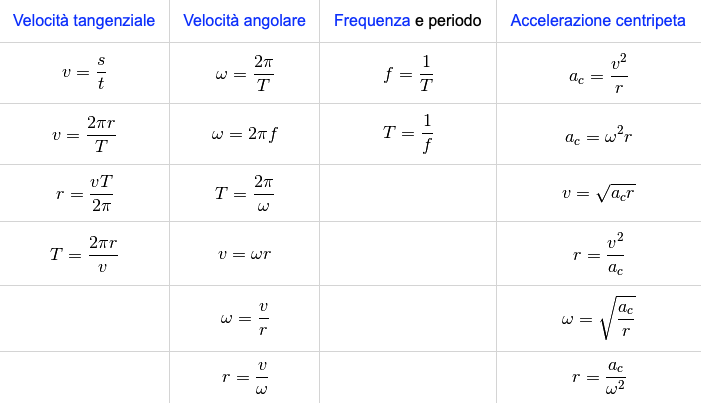
\includegraphics[width=0.9\linewidth]
        {formulario/img/Formulario_MCU.png}
        \caption{Formule del Moto circolare uniforme}
        \label{fig:MCU}
    \end{figure}

    \begin{figure}[H]
        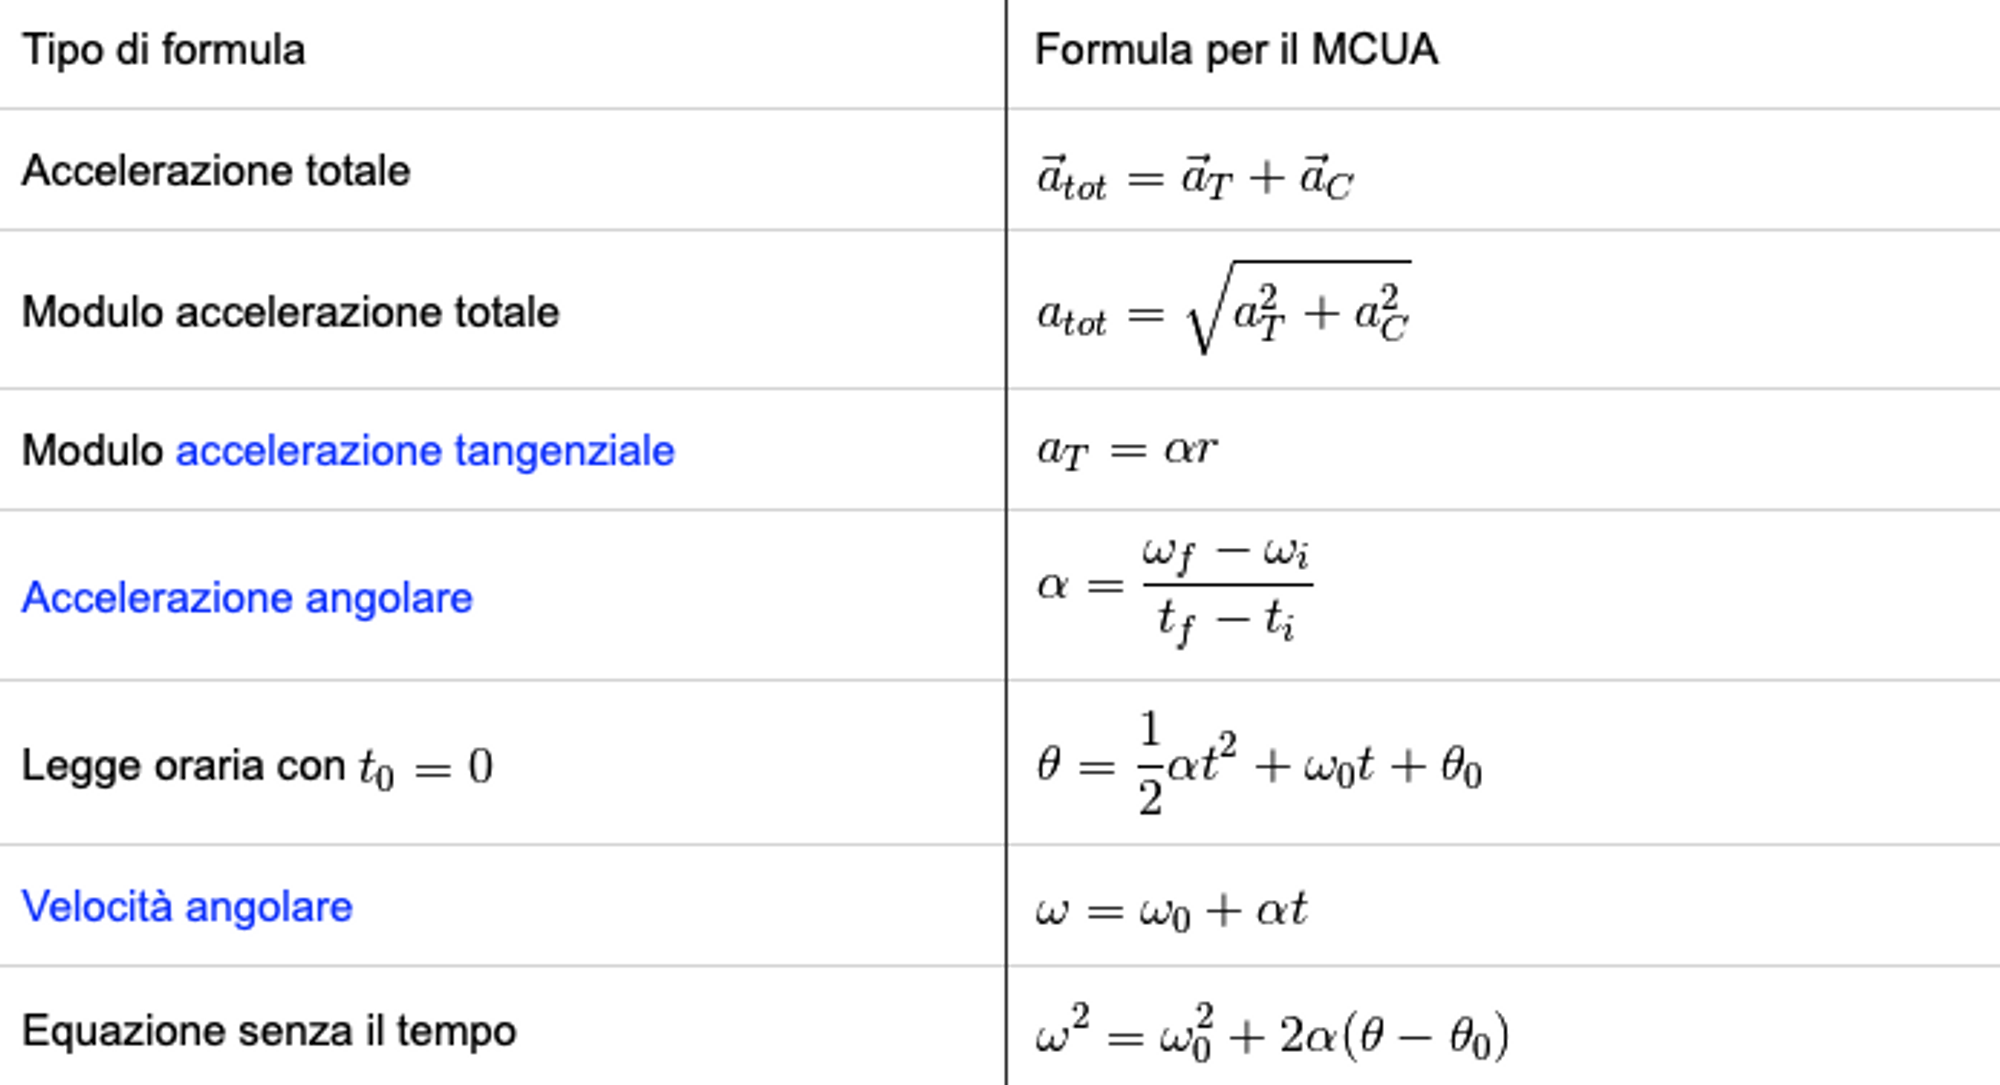
\includegraphics[width=0.9\linewidth]
        {formulario/img/Formulario_MCUA.png}
        \caption{Formule del Moto circolare uniformemente accelerato}
        \label{fig:MCUA}
    \end{figure}


\chapter*{Dinamica}

    \section*{Principi della Dinamica - Leggi di Newton}

        \subsection*{Prima Legge di Newton} Se la somma delle forze che agiscono 
        su un corpo è nulla, allora il corpo in quiete rimarrà in quiete, 
        mentre se è in moto, continuerà a muoversi di moto rettilineo uniforme.

        \subsection*{Seconda Legge di Newton} La forza agente su un corpo è 
        direttamente proporzionale all'accelerazione e ne condivide la 
        direzione e il verso, ed è direttamente proporzionale alla massa. Di 
        contro l'accelerazione cui è soggetto il corpo è direttamente 
        proporzionale alla forza e inversamente proporzionale rispetto alla 
        massa.

        \begin{equation*}
            \vec{F}_{net} = m \vec{a} \; \Bigg[N = \frac{Kg \cdot m}
            {s^2} \Bigg]
        \end{equation*}

        \subsection*{Terza Legge di Newton} Se un corpo A esercita una forza su 
        un corpo B, allora il corpo B esercita su A una forza uguale e 
        contraria.

        \begin{equation*}
            F_{ab} = - F_{ba}
        \end{equation*}

        \begin{quote}
            Attenzione! Le forze hanno modulo uguale ma con segno vettoriale 
            opposto!
        \end{quote}

    \section*{Forza Elastica}
        \begin{equation*}
            F = -kx
        \end{equation*}

    \section*{Carrucola}
        \begin{equation*}
            \begin{cases}
                F_{y1} = T - m_1g \\
                F_{y2} = m_2g - T
            \end{cases}
        \end{equation*}

    \section*{Attrito Statico e Dinamico}
        \begin{itemize}
            \item \textbf{Attrito statico}: agente quando il corpo è fermo, 
            impedendo lo spostamento iniziale.
            \item \textbf{Attrito dinamico}: agente da quando il corpo ha 
            appena compiuto lo spostamento iniziale ed è in movimento.
        \end{itemize}
    Le formule sono per l'attrito statico:
        \begin{equation*}
            f_{s, max} = \mu_sF_N \;\Bigg[N = \frac{Kg \cdot m} {s^2} \Bigg]
        \end{equation*}
        Mentre per quello dinamico:
        \begin{equation*}
            f_{k} = \mu_kF_N \;\Bigg[N = \frac{Kg \cdot m} {s^2} \Bigg]
        \end{equation*}
    
    \section*{Resistenza di un corpo}
        \begin{equation*}
            D = \frac{1}{2}CA\rho v^2
        \end{equation*}
        Con:
        \begin{itemize}
            \item C : Coefficiente di resistenza aerodinamica.
            \item A : Area efficace della sezione trasversale del corpo.
            \item $\rho$ : densità dell'aria
            \item v : velocità.
        \end{itemize}

    \section*{Lavoro}

        \begin{equation*}
            W = Fd = Fd \cos \Theta \;\Bigg[J = N \cdot m = 
            \frac{Kg \cdot m^2}{s^2}\Bigg]
        \end{equation*}

        \subsection*{Lavoro compiuto dalla Forza Gravitazionale}
            \begin{equation*}
                F = mgd\cos \Theta = mgd \cos 180 = - mgd
            \end{equation*}

        \subsection*{Lavoro compiuto dalla Forza Elastica} 
            \begin{equation*}
                W_m = \frac{1}{2}kx^2_i - \frac{1}{2}kx^2_f \;[J]
            \end{equation*}

    \section*{Energia Cinetica}
        \begin{equation*}
            K = \frac{1}{2}mv^2 \;[J]
        \end{equation*}

        \subsection*{Teorema dell'Energia Cinetica}
            \begin{equation*}
                \Delta K = K_f - K_i = W
            \end{equation*}

        \subsection*{Energia Cinetica del Moto Armonico Semplice}
            \begin{equation*}
                K = \frac{1}{2}mv^2 = \frac{1}{2}m\omega^2A^2\sin^2
                (\Theta + \omega t)
            \end{equation*}

    
    \section*{Potenza}
        \begin{equation*}
            P = \frac{W}{\Delta t} \; \Bigg[W \textsf{  Watt} = \frac{J}{s} 
            = \frac{Kg \cdot m^2}{s^2} \cdot \frac{1}{s} 
            = \frac{Kg \cdot m^2}{s^3} \Bigg]
        \end{equation*}
        \begin{equation*}
            P = \frac{dL}{dt} = \frac{F \cos \Theta dx}{dv} 
            = F \cos \Theta (\frac{dx}{dt})
        \end{equation*}
        Ma sappiamo benissimo che $\frac{dx}{dv}$ non è altro che la definzione 
        di velocità. Possiamo quindi riscriverla in modo più semplice:
        \begin{equation*}
            P = Fv\cos\Theta
        \end{equation*}
        Ovvero il \textbf{prodotto scalare} tra $F$ e $v$ (dove $v$ è la 
        velocità della particella). Possiamo quindi scrivere che la Potenza 
        Istantanea di una paricella a velocità $v$ non è altro che:
        \begin{equation*}
            P = F \cdot v
        \end{equation*}

    \section*{Energia Potenziale}
        \begin{equation*}
            \Delta U = - W \;[J]
        \end{equation*}

        \subsection*{Energia Potenziale Gravitazionale}
            \begin{equation*}
                \Delta U = mg(y_f - y_i) = mg \Delta y
            \end{equation*}

        \subsection*{Energia Potenziale Elastica}
            \begin{equation*}
                U(x)     = \frac{1}{2}kx^2
            \end{equation*}

        \subsection*{Energia Potenziale del Moto Armonico Semplice}
            \begin{equation*}
                U = \frac{1}{2}kx^2 = \frac{1}{2}kA^2\cos^2(\Theta + \omega t)
            \end{equation*}

    \section*{Energia Meccanica}
        \begin{equation*}
            E_m = K + U
        \end{equation*}

        \subsection*{Principio di conservazione dell'Energia Meccanica}
            \begin{equation*}
                \Delta E_m = \Delta K + \Delta U = 0
            \end{equation*}

        \paragraph{Principio esteso}
            \begin{equation*}
                \Delta E_m = W_{nc}
            \end{equation*}
        

    \section*{Moto Armonico e Pendolo} \ref{moto_armonico}
        \begin{equation*}
            x(t) = A \cos(\Theta_0 + \omega t)
        \end{equation*}
        ma con:
        \begin{equation*}
            \omega = \sqrt[]{\frac{k}{m}}
        \end{equation*}
        ricordando l'equazione dei un sistema molla-blocco:
        \begin{equation*}
            F = -kx
        \end{equation*}
        
        \paragraph{Il pendolo} Il pendolo può essere descritto tramite il
        Moto Circolare Uniformemente Accelerato:
        \begin{equation*}
            \omega = \sqrt[]{\frac{g}{L}}
        \end{equation*}
    
\newpage
    
    \section*{Momento Lineare}
        \begin{equation*}
            p = mv \; \Bigg[Kg \cdot \frac{m}{s}\Bigg] 
        \end{equation*}

    \section*{Impulso}
        \begin{equation*}
            I = \Delta p
        \end{equation*}

        \paragraph{Connessione con il Momento Lineare} Sia una forza $F = F(t)$
        agente su una particella. Applicando la II Legge di Newton:

        \begin{equation*}
            F = \frac{dp}{dt} \implies dp = F dt
        \end{equation*}
        \begin{equation*}
            \Delta p = p_f - p_i = \int_{t_f}^{t_i} F \,dt = I 
        \end{equation*}
    
    \section*{Urti}
    \begin{itemize}
        \item \textbf{Urti elastici}: Se nell'urto tra due corpi l'Energia 
        Cinetica totale del sistema non cambia ma si conserva completamente.
        \item \textbf{Urti anaelastici}: L'Energia Cinetica non si conserva ma 
        parte viene dispersa in calore o suono (ad esempio).
    \end{itemize} 

        \subsection*{Urti Anaelastici}
            \begin{equation*}
                p_{1,i} + p_{2,i} = p_{1,f} + p_{2,f}
            \end{equation*}
        ovvero:
            \begin{equation*}
                m_1v_{1,i} + m_2v_{2,i} = m_1v_{1,f} + m_2v_{2,f}
            \end{equation*}
        Nel caso di un \textbf{urto completamente anaelastico} uno dei due 
        corpi sarà inizalmente fermo (prendendo il nome di bersaglio):
        \begin{equation*}
            m_1v_{1,i} = (m_1+m_2)V
        \end{equation*}
        



\chapter*{Gravitazione}

\begin{equation*}
    F_g = G\frac{m_1m_2}{r^2} \; \Bigg[\frac{m^3}{\text{Kg}\cdot s^2} \cdot
    \frac{\text{Kg}^2}{m^2} = \frac{m \cdot \text{Kg}}{s^2} \Bigg]
\end{equation*}
Dove $G$ è la costante di gravitazione universale:
\begin{equation*}
    G = 6,673^{-11} \;\Bigg[\frac{m^3}{\text{Kg}\cdot s^2}\Bigg]
\end{equation*}

\begingroup
\setlength{\tabcolsep}{20pt} % Default value: 6pt
\renewcommand{\arraystretch}{2} % Default value: 1
\begin{tabular}{|c|c|}
    \hline Energia Potenziale Gravitazionale &
        $
        U_g = \frac{-GMm}{R}
        $
        \\

    \hline Velocità di Fuga &
        $
        v = \sqrt[]{\frac{2GM}{R}}
        $
        \\
    \hline
\end{tabular}
\endgroup

\chapter*{Fluidostatica}

    \section*{Pressione} 
        \begin{equation*}
            p = \frac{F}{A} \; \Bigg[Pa \textsf{ Pascal} = \frac{Kg}{m \cdot 
            s^2} \Bigg]
        \end{equation*}
    È uno scalare, proporizionale al modulo della forza.

    \section*{Densità}
        \begin{equation*}
            \rho = \frac{m}{V} \; \Bigg[\frac{Kg}{m^3}\Bigg]
        \end{equation*}
    Se $\rho$ è costante, il liquido preso in considerazione è incompressibile.

    \section*{Legge di Stevino} 
        \begin{equation*}
            p_2 = p_1 + \rho g(y_1-y_2)
        \end{equation*}
    Chiamiamo $h$ la profondità di un campione in un fluido misurata a partire
    da un livello di riferimento a cui la pressione assume un valore $p_0$, la 
    precedente equazione diventa:
        \begin{equation*}
            p = p_0 + \rho gh
        \end{equation*}
    In cui $p$ è la pressione alla profondità $h$.
    La pressione è la stessa per tutti i punti allo stesso livello.

    \section*{Forza di Bouyant}
        \begin{align}
            F_{archimede} &= m_{liquido}g \\
            F_a &= (\rho V) g
        \end{align}
        \subsection*{Oggetto totalmente sommerso} S
            \begin{equation*}
                F_g = M_g = (\rho_0 V_0) g
            \end{equation*}

        \subsection*{Oggetto galleggiante}
            \begin{align}
                F_a = F_g :
                \begin{cases}
                    F_a &= (\rho_f V_f)g \\
                    F_g &= M_g = (\rho_0 V_0)g
                \end{cases}
            \end{align}
        $F_a = F_g$ perché l'oggetto è in equilibrio.

    \section*{Peso appartente di un oggetto}
        \begin{equation*}
            P_{app} = P - F_a
        \end{equation*}
            

\chapter*{Fluidodinamica}

    \section*{Equazione di Continuità} 
        \begin{equation*}
            R_v = Av = \textsf{cost} \, \Bigg[\frac{m^3}{s}\Bigg]
        \end{equation*}
    $R_v$ prende il nome di \textbf{portata volumica}, con $A$ la sezione del 
    tubo in un qualsiasi punto e $v$ la velocità del fluido.
    Sappiamo che la massa di un fluido è data dalla seguente equazione:
        \begin{equation*}
            m = \rho V
        \end{equation*}
    Quindi moltiplicando la Portata Volumica per la densità del fluido 
    otterremo la \textbf{portata massica}, definita come:
        \begin{equation*}
            R_m = \rho R_v = \rho A v = \textsf{cost}
        \end{equation*}

    \section*{Equazione di Bernoulli} 
        \begin{equation*}
            p_1 + \frac{1}{2}\rho v^2_1 + \rho g y_1 
            =
            p_2 + \frac{1}{2}\rho v^2_2 + \rho g y_2 
            = 
            \textsf{cost}
        \end{equation*}
        \begin{quote}
            In un fluido a flusso laminare, la somma della pressione, 
            dell'Energia Cinetica per unitò di Volume e dell'Energia 
            Potenziale gravitazionale per unità di Volume è 
            \textbf{costante}.
        \end{quote}


\chapter*{Termodinamica}

    \section*{Principio Zero della Termodinamica} Se due corpi $A$ e $B$ si 
    trovano in equilibrio termico con un terzo corpo $T$, allora sono in 
    reciproco quilibrio termico.

    \section*{Dilatazione Termica}
            \begin{equation*}
                \Delta l = \alpha l \Delta T
            \end{equation*}
        Nella quale $\alpha$ è il \textbf{coefficiente di dilatazione lineare}.

        \subsection*{Dilatazione Volumica}
            \begin{equation*}
                \Delta V = \beta V \Delta T
            \end{equation*}
        dove $\beta = 3\alpha$ è il \textbf{coefficiente di dilatazione 
        volumica} della sostanza.

    \section*{Calore}
        \begin{equation*}
            1 \; cal = 4,1868 \; J
        \end{equation*}

        \subsection*{Capacità Termica}
            \begin{equation*}
                Q = C \Delta T = C (T_2 - T_1)
            \end{equation*}
        dove $C$ è la \textbf{capacità termica} dell'oggetto.

        \subsection*{Calore Specifico}
            \begin{equation*}
                Q = cm \Delta T
                \implies
                c = \frac{Q}{m \Delta T}
             \; \Bigg[\frac{J}{K \cdot Kg}\Bigg]
            \end{equation*}

        \subsection*{Calore Latente}
            \begin{equation*}
                Q = Lm \implies L = \frac{Q}{m}
            \end{equation*}
        Il \textbf{calore latente di evaporazione} $L_v$ è la quantità di 
        energia per unità di massa che deve essere fornita per far evaporare un
        liquido o che deve essere \textbf{sottratta} per liquefare un gas. Il 
        \textbf{calore latente di fusione} $L_f$ è la quantità di energia per 
        unità di massa ched eve essere fornita per fondere un solido o che deve
        essere sottratta per solidifcare un liquido.
        
    \section*{Lavoro associato ad una variazione di Volume} 
        \begin{equation*}
            L = \int_{V_i}^{V_f} dL =  \int_{V_i}^{V_f} p \,dV  
        \end{equation*}
    L'integrazione è necessaria perché la pressione $p$ può cambiare durante la
    varizione del volume.

    \section*{Primo Principio della Termodinamica}
        \begin{align*}
            \Delta E_{int} &= E_{int, f} - E_{int, i} = \Delta Q - \Delta W \\
            d E_{int} &= d Q - d W
        \end{align*}

        \subsection*{Applicazioni del Primo Principio} Il primo principio della 
        termodinamica trova applicazione in numerosi casi particolari, tra cui:
            \begin{itemize}
                \item \textit{Trasformazioni Isocore ($V$ costante)}:
                    $W = 0 \implies \Delta E_{int} = \Delta Q$
                \item \textit{Trasformazioni Isobara ($p$ costante)}:
                    $W = p(V_2-V_1)$, $Q = nc_p\Delta T$
                \item \textit{Trasformazioni Isoterma ($T$ costante)}:
                    $pV = \text{cost}$, $W = nRT\ln(\frac{V_f}{V_i})$, 
                    $\Delta E_{int} = 0 \; Q = + W$
                \item \textit{Trasformazioni Cicliche}:
                    $\Delta E_{int} = 0 \implies \Delta Q = \Delta W$
                \item \textit{Trasformazioni ad Espansione Libera}: si tratta 
                        di trasformazioni adiabatiche nelle quali non viene 
                        compiuto alcun lavoro sul sistema o da parte di esso.
                        Ad esempio se abbiamo due contenitori collegati isolati 
                        dall'esterno. Nel primo c'è un gas mentre il secondo è
                        vuoto. Nel momento in cui apriamo il rubinetto che 
                        collega i due, il gas inizia ad occupare lo spazio 
                        vuoto ma non cambiando calore non compie lavoro 
                        (siccome ci troviamo in un sistema isolato), inoltre,
                        la sua espansione non è contratasta da alcuna pressione
                        . Siamo quindi nella seguente situazione:
                        $\Delta Q = \Delta L = 0 \implies \Delta E_{int} = 0$
                \item \textit{Trasformazioni Adiabatiche}: 
                        $Q=0 \implies \Delta E_{int} = -\Delta W \;
                        pV^\gamma = \text{cost}
                        $ con $\gamma = \frac{c_p}{c_v} \implies c_p = c_v + R
                        \implies \gamma = \frac{c_v + R}{c_v}$. Ricodiamo 
                        inoltre che $c_v = $ (per tipo di gas):
                        \begin{itemize}
                            \item Monoatomico: $\frac{3}{2} R$
                            \item Biatomico: $\frac{5}{2} R$
                            \item Poliatomico: $3 R$
                        \end{itemize}
            \end{itemize}

        \section*{Conduzione, Convezione ed Irraggiamento} 

            \subsection*{Conduzione}
                \begin{equation*}
                    P_c = \frac{Q}{t} = kA\frac{T_1 - T_2}{l}
                \end{equation*}

            \paragraph{Resistenza termina alla conduzione}
                \begin{equation*}
                    R = \frac{l}{k}
                \end{equation*}

            \subsection*{Convezione} La convezione ha luogo quando le differenze
            di temperatura causano il moto che trasferisce calore all'interno 
            di un fluido.

            \subsection*{Irraggiamento}
                \begin{equation*}
                    P_r = \sigma \epsilon AT^4
                \end{equation*}
            Dove $\sigma = 5,6703 \cdot 10^{-8} \; [\frac{W}{m^2 \cdot K^4}
            ]$ è la costante di Stefan-Boltzmann, $\epsilon$ è l'emittanza
            caratteristica della superficie, $A$ è l'area irraggiante e $T$ la 
            temperatura superficiale in Kelvin. La potenza $P_a$ che un oggetto
            assorbe per via radiativa dell'ambiente a temperatura uniforme
            $T_{amb}$ (in Kelvin) è:
                \begin{equation*}
                    P_a = \sigma \epsilon AT^4_{amb}
                \end{equation*}

    \section*{Numero di Avogadro}
        \begin{equation*}
            N_a = 6,022 \cdot 10^{23}
        \end{equation*}

        \subsection*{Massa molare}
            \begin{equation*}
                M = mN_a
            \end{equation*}
        
        \subsection*{Numero di moli}
            \begin{equation*}
                n = \frac{N}{N_A} = \frac{M_{cam}}{M} = \frac{M_{cam}}{mN_A}
            \end{equation*}

    \section*{Gas ideale o Gas perfetti} 
        \begin{equation*}
            pV = nRT
        \end{equation*}
    Con:
        \begin{itemize}
            \item $p$ Pressione del cilindro.
            \item $n$ Numero di moli.
            \item $R$ Costante dei gas $= 8,31 \; \frac{J}{mol \cdot K}$
            \item $T$ Temperatura del cilindro.
        \end{itemize}
    Questa legge si può scrivere anche come:
        \begin{equation*}
            pV = NkT
        \end{equation*}
    Dove $k$ è la costante di Boltzmann e vale:
        \begin{equation*}
            k = \frac{R}{N_A} = 1,38 \cdot 10^{-23} \; \Bigg[\frac{J}{K}\Bigg]
        \end{equation*}
        \subsection*{Equazione di stato per i gas ideali DA VERIFICARE}
            \begin{equation*}
                (p + \frac{an^2}{v^2})(V - nb) = nRT
            \end{equation*}

    \section*{Pressione, temperatura e velocità molecolare}
            \begin{equation*}
                p = \frac{nMv^2_{qm}}{3V}
            \end{equation*}
    Dove $v_{qm} = \sqrt[]{v^2}$ è la \textbf{velocità quadratica media} delle
    molecole del gas. Con l'equazione dei gas perfetti si ha:
            \begin{equation*}
                v_{qm} = \sqrt[]{\frac{3RT}{M}}
            \end{equation*}

\chapter*{Elettrostatica}

    \section*{Legge di Coulomb}
        \begin{equation*}
            F = k\frac{q_1q_2}{r^2}\widehat{r}
        \end{equation*}
    Con:
    \begin{equation*}
        k = \frac{1}{4\pi\varepsilon_0}
    \end{equation*}
    Sostituendo nella Legge di Coulomb otteniamo:
    \begin{equation*}
        F = \frac{1}{4\pi\varepsilon_0}\frac{q_1q_2}{r^2}\widehat{r}
    \end{equation*}
    con $\varepsilon_0 = 8,85\cdot 10^{-12}\;C^2/(N\cdot m^2)$.
        \subsection*{Principio di sovrapposizione}
        Se su una particella agiscono più forze di carica, la $F_{tot}$ non 
        sarà altro che la somma vettoriale di tutte le forze!

        \subsection*{Corrente elettrica}
            \begin{equation*}
                i = \frac{dq}{dt} \; [A \cdot s]
            \end{equation*}
    
        \subsection*{La carica è quantizzata} 
            \begin{equation*}
                q = ne
            \end{equation*}
        dove $e = 1,602\cdot10^{-19} [C]$ è la cosstante elementare, una delle
        costanti fondamentali della materia.
        \begin{center}
            \begin{tabular}{ |c|c| } 
                \hline
                Particella & Carica \\
                \hline
                Elettrone & $- e$ \\
                Positrone & $+ e$ \\
                Protone & $+ e$ \\
                Antiprotone & $- e$ \\
                quark & $\pm \frac{1}{3}e \;\; \pm \frac{2}{3}e$ \\
                Neutrone & $0$ \\
                \hline
            \end{tabular}
        \end{center}

        \section*{Campo Elettrico}
            \begin{equation*}
                E = \frac{F}{q_0}\;\Bigg[\frac{N}{C}\Bigg]
            \end{equation*}

            \subsection{Campo elettrico generato da una carica puntiforme}
                \begin{equation}
                    E = \frac{1}{4\pi\varepsilon_0}\frac{|q|}{r^2}
                \end{equation}

            \subsection*{Principio di sovrapposizione} 
                \begin{equation*}
                    E = \frac{F_0}{q_0} = \frac{F_{01} + F_{02} + \cdots + 
                    F_{0n}}{q_0} = E_1 + E_2 + \cdots + E_n
                \end{equation*}

            \subsection*{Densità del campo elettrico} 
            \begin{itemize}
                \item \textit{Densità di carica lineare} $\lambda$: numero di 
                cariche per unità di lunghezza.\\
                    \begin{equation*}
                        \lambda = \frac{Q}{m}
                    \end{equation*}
                \item \textit{Densità di carica superficiale} $\sigma$: numero 
                di cariche per unità di superifice.\\
                    \begin{equation*}
                        \sigma = \frac{Q}{m^2}
                    \end{equation*}
                \item \textit{Densità di carica volumetrica} $\rho$: numero
                di cariche per unità di volume.\\
                    \begin{equation*}
                        \rho = \frac{Q}{m^3}
                    \end{equation*}
            \end{itemize}

        \section*{Flusso di Campo Elettrico}
            \subsection*{Caso 1: superficie piana e parallela con campo $E$
            uniforme}
                \begin{equation*}
                    \Delta\phi = E \Delta A = E \Delta A \cos\Theta 
                \end{equation*}
            Che sull'interezza della superficie diventa:
                \begin{equation*}
                \phi = \int E\cos\Theta \,dA  = E\cos\Theta\int\,dA = E\cos
                \Theta A 
                \end{equation*}
            \subsection*{Caso 2: superficie chiusa e campo $E$ uniforme}
                \begin{equation*}
                    \phi = \oint E \,dA
                \end{equation*}
        L'unità di misura del flusso è la seguente:
                \begin{equation*}
                    [\phi] = [E][A] = [N] \frac{[m^2]}{[C]}
                \end{equation*}
         
        \section*{Teorema di Gauss}
            \begin{equation*}
                \phi = \oint E \, dA = \frac{Q}{\varepsilon_0}
            \end{equation*}
        Non hanno alcuna importanza la dimensione e al forma della superficie,
        l'importante è che sia chiusa.

            \subsection*{Campo elettrico generato da un filo conduttore 
            infinitamente lungo}
                \begin{equation*}
                    E \cdot 2\pi rh = \frac{\lambda h}{\varepsilon_0}
                    \implies
                    E = \frac{\lambda}{2\pi\varepsilon_0r}
                \end{equation*}

            \subsection*{Campo elettrico esterno generato da un conduttore}
                \begin{equation*}
                    E = \frac{\sigma}{\varepsilon_0}
                \end{equation*}

        \section*{Potenziale Elettrico}
            \begin{equation*}
                V = \frac{-W_\infty}{q_0} = \frac{U}{q_0}
            \end{equation*}

            \subsection*{Energia Potenziale Elettrica}
                \begin{equation*}
                    U = qV
                \end{equation*}
            Se la particella si sposta subendo una variazione di potenziale 
            $\Delta V$, la variazione di energia potenziale elettrica è:
                \begin{equation*}
                    \Delta U = q \Delta V = q (V_f - V_i)
                \end{equation*}
            
        \section*{Energia Meccanica}
            \begin{equation*}
                \Delta K = -q \Delta V
            \end{equation*}
        Se al contrario è presente una forza applicata che compie lavoro 
        $w_{app}$ su di essa, la variazione di energia cinetica diventa:
            \begin{equation*}
                \Delta K = -q\Delta V + W_{app}
            \end{equation*}
        Nel caso particolare in cui $\Delta K = 0$:
            \begin{equation*}
                W_{app} = q \Delta V
            \end{equation*}

        \section*{Superfici Equipotenziali}
            \subsection*{Calcolo di $V$ a partire da $E$}
                \begin{equation*}
                    V_f - V_i = - \int_{i}^{f} E \,ds
                \end{equation*}
            Se il punto iniziale è posto all'infinito e $V_i = 0$ si ha, per il
            potenziale in un punto:
                \begin{equation*}
                    V = -\int_{i}^{f} E \,ds
                \end{equation*}
            Nel caso particolare di un campo uniforme di modulo $E$, la 
            differenza di potenziale tra le due linee equipotenziali adiacenti
            (necessariamente parallele) separate da una distanza $\Delta x$ è 
            data da:
                \begin{equation*}
                    \Delta V = -E\Delta x
                \end{equation*}

        \section*{Potenziale generato da cariche puntiformi}
            \begin{equation*}
                V = \frac{1}{4\pi\varepsilon_0}\frac{q}{r}
            \end{equation*}
        dove $q$ ha lo stesso segno di $V$. Il potenziale dovuto a una 
        distribuzione di cariche puntiformi è:
            \begin{equation*}
                V = \sum_{i = 1}^{n}V_i = \frac{1}{4\pi\varepsilon_0}
                \sum_{i = 1}^{n}\frac{q_i}{r_i}
            \end{equation*}

        \section*{Potenziale elettrico generato da una carica continua}
            \begin{equation*}
                V = \frac{1}{4\pi\varepsilon_0}\int \frac{dq}{r}
            \end{equation*}
        dove l'integrale è esteso all'intera distribuzione.

        \section*{Calcolo di $E$ partendo da $V$}
            \begin{equation*}
                E_s = - \frac{\partial V}{\partial s}
            \end{equation*}
        Si possono definire le componenti di $E$ secondo $x$, $y$ e $z$ nel 
        seguente modo:
            \begin{align*}
                E_x &= - \frac{\partial V}{\partial x}\\
                E_y &= - \frac{\partial V}{\partial y}\\
                E_z &= - \frac{\partial V}{\partial z}
            \end{align*}
        Se il campo $E$ è uniforme, la prima equazione si riduce a:
            \begin{equation*}
                E = - \frac{\Delta V}{\Delta s}
            \end{equation*}

        \section*{Energia Potenziale di un sistema di cariche puntiformi} 
            \begin{equation*}
                U = L = \frac{1}{4\pi\varepsilon_0}\frac{q_1q_2}{r}
            \end{equation*}

\chapter*{Elettrodinamica}

    \section*{Condensatori}
        \subsection*{Capacità di un condensatore}
            \begin{equation*}
                q = C\Delta V\;[F]
            \end{equation*}
        con $C$ costante di proporzionalità dipendente dalla geometria del 
        condesaotre. Indica capacità elettrica del condensatore.
        
        \subsection*{Calcolo della capacità elettrica di un condensatore} 
        Procedimento generale:
            \begin{itemize}
                \item Si assume che ci sia una carica $q$ sui piatti.
                \item Si calcola $E$ tra i due piatti in funzione di $q$, con 
                la legge di Gauss.
                \item Si calcola $\Delta V$ a partire da $E$
                \item Si calcola $C$
            \end{itemize}
        
        \subsection*{Capacità elettrica di un condensatore piano}
            \begin{equation*}
                C = \frac{\varepsilon_0A}{d}
            \end{equation*}

        \subsection*{Capacità elettrica di un condensatore cilindrico}
            \begin{equation*}
                C = \frac{q}{\Delta V} \implies C = \frac{2\pi\varepsilon_0L}
                {\ln(\frac{b}{a})}
            \end{equation*}

        \subsection*{Capacità elettrica di un condensatore sferico}
            \begin{equation*}
                C = \frac{q}{\Delta V} \implies C = 4\pi\varepsilon_0
                    \frac{ab}{b-a}
            \end{equation*}
        La capacità per una \textit{sfera isolata} di raggio r sarà:
            \begin{equation*}
                C = 4\pi\varepsilon_0r
            \end{equation*}
    
    \section*{Condensatori in Serie e Parallelo} 
        \subsection*{Condensatori in Parallelo}
            \begin{equation*}
                C_{eq} = \sum_{j = 1}^{n} C_j
            \end{equation*}

        \subsection*{Condensatori in Serie}
            \begin{equation*}
                \frac{1}{C_{eq}} = \sum_{j = 1}^{n} \frac{1}{C_j}
            \end{equation*}

    \section*{Energia potenziale di un condensatore}
        \begin{equation*}
            U = \frac{q^2}{2C} = \frac{1}{2}CV^2
        \end{equation*}
    La \textbf{densità di energia} $u$, ossia l'energia potenziale per unità di
     volume, è data da:
        \begin{equation*}
            u = \frac{1}{2}\varepsilon_0E^2
        \end{equation*}
    
    \section*{Capacità in presenza di un dielettrico}
        
        \subsection*{LEgge di Gauss in presenza di un dielettrico}
            \begin{equation*}
                \varepsilon_0 \oint \varepsilon_rR\cdot\,dA = q
            \end{equation*}

    \section*{Corrente elettrica}
        \begin{equation*}
            i = \frac{dq}{dt} \; \Bigg[A = \ \frac{C}{s}\Bigg]
        \end{equation*}

        \subsection*{Densità di corrente elettrica}
            \begin{equation*}
                i = \int J \, dA
            \end{equation*}
        
    \section*{Resistenza}
        \begin{equation*}
            R = \frac{V}{i} \; \Bigg[1 \Omega = 1 \frac{V}{A}\Bigg]        
        \end{equation*}
        
        \subsection*{Resistività e conducibilità}
            \begin{equation*}
                \rho = \frac{E}{J} = \frac{1}{\sigma}
            \end{equation*}

        \subsection*{Resistenza in Serie}
            \begin{equation*}
                R_{eq} = \sum_{j=1}^{n} R_j
            \end{equation*}

        \subsection*{Resistenza in Parallelo}
            \begin{equation*}
                \frac{1}{R_{eq}} = \sum_{j = 1}^{n} \frac{1}{R_j}
            \end{equation*}


    \section*{Legge di Ohm} La legge di Ohm asserisce che la corrente che scorre
    attraverso un dispositivo è \textit{sempre} direttamente proporizionale 
    alla differenza di potenziale applicata al dispositivo stesso

    \section*{Potenza nei Circuiti Elettrici}:
        \begin{equation*}
            P = iV
        \end{equation*}

    \section*{Forza elettromotrice di un generatore di Tensione}
        \begin{equation*}
            \xi = \frac{dW}{dq} \; [V]   
        \end{equation*}

    \section*{Analisi dei circuiti} La variazione di potenziale attraverso una 
    resistenza nella direzione della corrente è $-iR$; nella direzione opposta
    è $+iR$. La variazione di potenziale attraverso una generatore f.e.m ideale
    nella direzione della freccia della f.e.m è $+\xi$; nella direzione opposta
    è $-\xi$. Il principio di conservazione dell'energia porta alla legge delle
    maglie (secondo principio di Kirchoff).

    \section*{Legge delle maglie} \textit{La somma algebrica delle variazioni di
    potenziale incontrate in un giro completo di un qualsiasi circuito deve 
    essere uguale a zero}.\\
    La conservazione della carica si esprime nella legge dei nodi (primo 
    principio di Kirchoff).

    \section*{Legge dei nodi} \textit{La somma algebrica delle variazioni di 
    potenziale che si dipartono da qualsiasi nodo deve essere uguale alla somma
    delle correnti che giungono allo stesso nodo}.

    \section*{Circuiti RC}
        \begin{equation*}
            q = C\xi(1-e^{\frac{-t}{RC}})
        \end{equation*}
    nella quale $C\xi = q_0$ è la carica all'equilibrio e $RC = \tau$ è la 
    \textbf{costante di tempo capacitiva} del circuito. Durante la carica la 
    corrente è:
        \begin{equation*}
            i = \frac{dq}{dt} = (\frac{\xi}{R})e^{\frac{-t}{RC}}
        \end{equation*}
    Quando un condensatore si scarica attraverso una resistenza $R$, la carica
    del condensatore decade secondo l'espressione:
        \begin{equation*}
            q = q_0e^{\frac{-t}{RC}}
        \end{equation*}
    Durante la scarica la corrente è:
        \begin{equation*}
            i = \frac{dq}{dt} = -\frac{q_0}{RC}e^{\frac{-t}{RC}}
        \end{equation*}


\chapter*{Elettromagnetismo}

    \section*{Forza di Lorentz}
        \begin{equation*}
            F_B = qv \times B = qvB\sin\Theta \; [T]
        \end{equation*}

    \section*{Carica in moto circolare uniforme}
        \begin{equation*}
            |q|vB = \frac{mv^2}{r}
        \end{equation*}
    da cui troviamo il raggio:
        \begin{equation*}
            r = \frac{mv}{|q|B}
        \end{equation*}
    La frequenza di rivoluzione $f$, la pulsazione $\omega$ e il periodo $T$
    sono dati da:
        \begin{equation*}
            f = \frac{\omega}{2\pi} = \frac{1}{T} = \frac{|q|B}{2\pi m}
        \end{equation*}

    \section*{Forza agente su un filo percorso da corrente}
        \begin{equation*}
            F_B = iL\times B
        \end{equation*}
    La forza agente su un elemento infinitesimo $idL$ in un campo magnetico è:
        \begin{equation*}
            dF_B = idL\times B
        \end{equation*}

    \section*{Campo Magnetico generato da una corrente elettrica}

        \subsection*{Legge di Biot-Savart}
            \begin{equation*}
                dB = \Bigg(\frac{\mu_o}{4\pi}\Bigg)\frac{ids\times r}{r^3}
            \end{equation*}
        In questo caso r è il vetore diretto dall'elemento di corrente verso il
        punto in questione. La quantità chiamata $\mu_0$, chiamata costante di 
        permeabilità magnetica nel vuoto, ha un valore pari a $4\pi \cdot 
        10{^-7} = 1,26 \cdot 10^{-6} T \frac{m}{A}$.

        \subsection*{Campo magnetico in un filo lungo rettilineo}
            \begin{equation*}
                B = \frac{\mu_0i}{2\pi r}
            \end{equation*}

        \subsection*{Campo magnetico in un filo piegato ad arco}
            \begin{equation*}
                B = \frac{\mu_0i\phi}{4\pi R}
            \end{equation*}
        
        \subsection*{Forza tra due fili conduttori paralleli}
            \begin{equation*}
                F_{ba} = i_bLB_a\sin90 = \frac{\mu_0Li_ai_b}{2\pi d}
            \end{equation*}

    \section*{Legge di Ampere} La legge di Ampere afferma:
        \begin{equation*}
            \oint B \, ds = \mu_0i_{ch}
        \end{equation*}

    \section*{Solenoide}
        \begin{equation*}
            B = \mu_0in
        \end{equation*}
    dove $n$ è il numero delle spire per unità di lunghezza. Perciò il campo 
    magnetico interno è uniforme.

\end{document}